\chapter{Earthquake source generation}
\label{ch:source}

\section{Overview}

The EQRM conducts probabilistic seismic hazard analysis (PSHA) and
probabilistic seismic risk analysis (PSRA) using an event based
approach. This means that the ground motions (hazard) and loss
(risk) are computed for each event individually and the results
separately aggregated to form probabilistic estimates. The event
based approach differs from the traditional approach to PSHA which
integrates over all magnitude and distance combinations to attain
probability levels for exceeding a particular level of ground
motion in a pre-defined period of time. The traditional approach
is introduced by \citet{dr_Cornell68a} and summarised by
\citet{dr_McGuire90a}, while the event based approach is outlined by \citet{eqrm_Musson00}. A core component of any event based
analysis with the EQRM is the generation of a simulated
event \index{simulated event} catalogue. The
generation of the event catalogue relies upon an existing model for
the seismicity in the region. Typically the  model of seismicity comes
 from an interpretation of historical earthquakes,
 geology and neotectonics. The current version of the EQRM application requires a source model
that consists of a set of areal source zones (defined by a polygon) and/or fault sources (defined by a plane). Users can use either a bounded Gutenberg-Richter 
or characteristic earthquake model \citep{eqrm_Schwartz84} 
to describe the earthquake recurrence relationships. 

\emph{Areal source zones} capture the background seismicity in an area and are decribed by the acitivty rate within
each source zone through its Gutenberg-Richter \emph{b} value and $A_{min}$ (the number of earthquakes per year greater than $M_{min}$). 
In event-based PSHA calculations, such as the EQRM,
synthetic ruptures will be generated stochastically throughout an areal source zone. However, a user may have sufficient information 
on the geometry and earthquake recurrence rates of a known fault and may want to place synthetic ruptures on the fault by defining a 
\emph{fault source}. In this instance, instead of placing the synthetic ruptures within the areal source zone, they will be restricted to a particular fault plane. 

In addition, a novel technique has been developed to generate synthetic ruptures within a dipping 3D volume that may represent seismotectonic 
features such as the intraslab of a subducting slab, therefore allowing the EQRM to realistically simulate \emph{intraslab ruptures}.

This chapter describes the process of creating a synthetic earthquake catalogue and for defining an individual scenario event. 
The chapter is organised as follows. First, the concept of a synthetic earhquake catalogue is discussed (Section \ref{sec:source-EQcat} and \ref{sec:source-virtual_faults}), 
then the approach for 
determining earthquake magnitudes and recurrence rates is presented in Section \ref{sec:magnitude_selection}. This is followed by a
description of the method for generating realistic synthetic ruptures in areal source zones (Section \ref{sec:areal_gen}) or on a predefined fault (Section \ref{sec:fault_gen}). 
Section \ref{source:spawning} discusses the concept of spawned events which is used to produce spatially correlate ground motions. Lastly, Section \ref{sec:source-scenario} describes the approach for scenario event generation.

\section{Creating an earthquake catalogue for probabilistic seismic hazard analysis}% a probabilistic seismic hazard analysis}
\label{sec:source-EQcat}

This section describes the method to generate a synthetic catalogue of plausible events. The event catalogue can be
created for events that are defined within an areal source zone or located on a known fault. The recurrence relationship for the events
can be defined as a bounded Gutenberg-Richter \citep{dr_Kramer96a} or characteristic earthquake \citep{eqrm_Schwartz84} relationships.

A simulated event is represented by a 2D plane
(or rupture) in 3D space that signifies the region where slip has
occurred. The parameters descibing the geometry of a rupture plane are shown in
\Fref{fig:hrupture-3d}. The important parameters of a simulated
event\index{simulated event} are its location, geometry, magnitude
and activity (or likelihood of occurrence). The rupture trace is
the surface projection of the simulated event\index{simulated
event} along the direction of dip. The position and geometry of
the rupture trace is defined by its start $(r_s^{lat},r_s^{lon})$
and end $(r_e^{lat},r_e^{lon})$ points, its azimuth $r_{azi}$ and
its length $r_l$. The position and geometry of the rupture plane
are defined by its width ($r_w$), dip ($r_{dip}$) and the position of
its centre (or rupture centroid). The ruputre plane dips to the right of the fault trace when looking along the trace. 
The rupture centroid is defined
in cartesian coordinates $(r_x,r_y,r_z)$ in km using a local
coordinate system with origin at the rupture start point (see
\Fref{fig:hrupture-3d}). The orientation of the local coordinate
system is such that the $x-axis$ is oriented along the rupture
trace with positive direction pointing towards the rupture end
point, the $z-axis$ is pointing vertically downwards and the
$y-axis$ is oriented along the surface of the Earth such that
the axes form a right handed triad. The vertical projection of the
rupture centroid is also described by its latitude $r_c^{lat}$ and
longitude $r_c^{lon}$. The ruptures are not allowed to extend above the surface of the Earth.
The event magnitude is represented as a
moment magnitude and is generated by the process described in
\sref{sec:magnitude_selection}. The activity (or likelihood of
occurrence) of the simulated event\index{simulated event} is
described by the event activity ($r_v$) which represents the number of
times a given simulated event\index{simulated event} (conditional
on magnitude and position) occurs in one year (see
\sref{sec:magnitude_selection}).

\begin{figure}[htp]
\begin{center}
\begin{tabular}{ll}
(a) & (b) \\
% \psfrag{Fault Trace}{Rupture Trace} \psfrag{Dip}{$r_\theta$}
% \psfrag{Azimuth}{$r_\phi$}
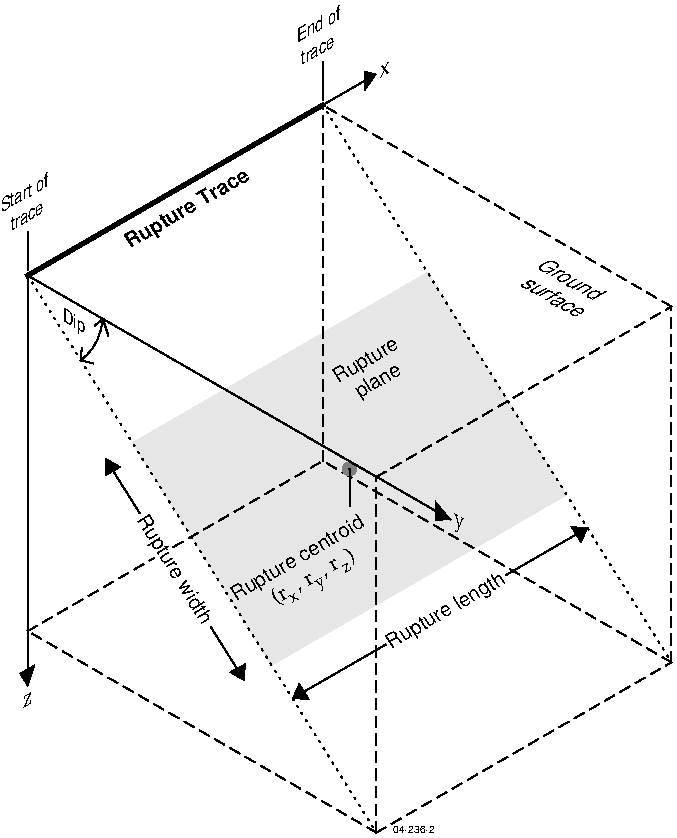
\includegraphics[width=0.49\textwidth]{diags/fig-hrupture-3d} &
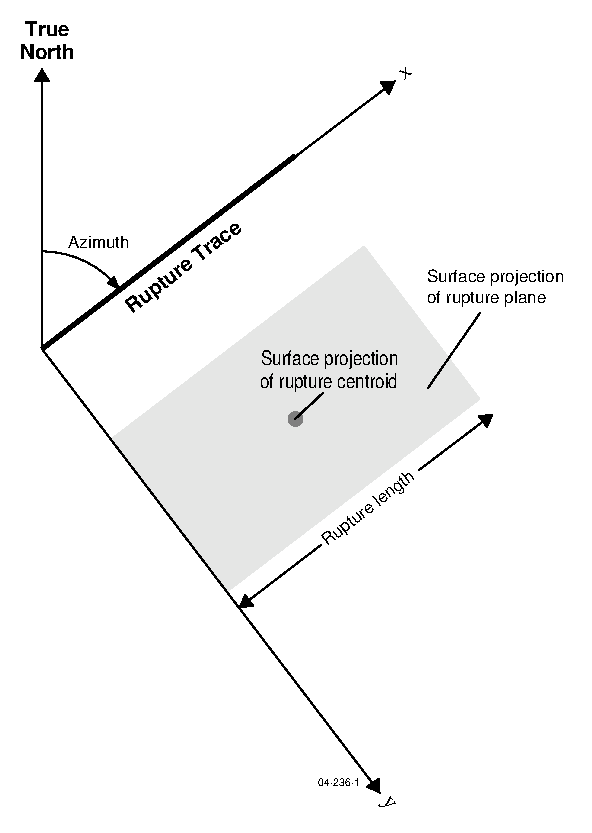
\includegraphics[width=0.41\textwidth]{diags/fig-hrupture-2d}
\end{tabular}
\end{center}
\caption{Orientation and dimension of the rupture plane in (a) 3D
and (b) 2D vertical projection to ground surface.}
\label{fig:hrupture-3d}
\end{figure}


\begin{table}
\caption{Definition of parameters used in generation of the synthetic earthquake catalogue.}
 \label{tab:parameters}
\begin{tabular}{l |  l}
\hline
Parameter & Definition \\
\hline \hline
$f_A$ & Fault area \\
$f_w$ & Fault width \\ 
$f_l$ & Fault length \\
$f_\phi$ & Fault azimuth \\
$f_\theta$ & Fault dip \\
$f_s^{lon}$ & Longitude of start of fault trace \\
$f_s^{lat}$ & Latitude of start of fault trace \\
$f_e^{lon}$ & Longitude of end of fault trace \\
$f_e^{lat}$ & Latitude of end of fault trace \\
$f_z^{top}$ & The top of the seismogenic zone \\
$f_z^{bot}$ & The bottom of the seismogenic zone \\ 
$r_A$ & Rupture area \\
$r_w$ & Rupture width \\
$r_l$ & Rupture length \\
$r_s^{lon}$ & Longitude of start of rupture trace \\
$r_s^{lat}$ & Latitude of start of rupture trace \\
$r_e^{lon}$ & Longitude of end of rupture trace \\
$r_e^{lat}$ & Latitude of end of rupture trace \\
$r_x$ & Rupture centroid x in local coordinate system \\ 
& (distance in km along rupture trace from start of fault trace) \\
$r_y$ & Rupture centroid y in local coordinate system \\ 
& (distance in km perpendicular from rupture trace in direction of dip) \\
$r_z$ & Rupture centroid depth (km) \\
$r_c^{lon}$ & Longitude of rupture centroid \\
$r_c^{lat}$ & Latitude of rupture centroid \\
$r_\phi$ & Rupture azimuth (degrees from true North) \\
$r_\theta$ & Rupture dip (degrees from horizontal) \\
$f_z^{top}$ & The upper limit of the seismogenic zone \\
$f_z^{bot}$ & The lower limit of the seismogenic zone \\ 
$\delta_\theta$ & Out of dip theta of rupture plane \\
$\Delta_\theta$ & Range of dips to be sampled either side of rupture plane \\
$s_w$ & Width of slab for intraslab events. This is used to constrain the \\
& out-of-plane ruptures \\
$A_{min}$ & number of earthquake of magnitude $M_{min}$ or greater per year. \\
$r_m$ & The event magnitude  \\ 
$r_v$ & The event activity, the number of magnitude $r_m$ earthquakes \\
& expected per year scaled to the number being simulated. \\
$r_\epsilon$ & Source epsilon from spawning. \\
$w_e$ & Weight derived from event spawning. \\
\hline
\end{tabular}
\end{table}


\section{Simulated events and virtual faults}
\label{sec:source-virtual_faults}

The terms simulated event\index{simulated event}, simulated
earthquake\index{simulated earthquake} and simulated
rupture\index{simulated rupture} are congruent and will be used
interchangeably throughout this document. Sometimes the adjective
`simulated' will be omitted for brevity. An adjective `actual'
will be used in place of `simulated' to refer to a historic
earthquake (i.e. one that has actually occurred rather than one
that is simulated).

A virtual fault\index{virtual fault} refers to a plane in 3D space upon which an event can
occur.  The virtual fault can be located within an areal source zone or defined by a known fault. 
The EQRM works by first creating a virtual fault\index{virtual fault}, either within an
areal source zone, or by a user defined fault. The rupture is then placed 
on the virtual fault\index{virtual fault} (the
rupture is not allowed to exceed the bounds of the virtual
fault\index{virtual fault}). The introduction of a virtual
fault\index{virtual fault} is the mechanism by which the
EQRM application constrains the location and extent
of each rupture. The depth to the top of a virtual
fault\index{virtual fault} is defined as the depth to the
seismogenic region $f_z$ (see
\tref{tab:parameters}). Other geometrical parameters
of virtual fault\index{virtual fault}s include the width $f_w$ and
length $f_l$. 


\section{Magnitude selection and event activity}
\label{sec:magnitude_selection}

A `stratified' Monte-Carlo technique is used to assign the event
magnitudes. The stratified nature of the technique ensures that
the full range of magnitudes is adequately sampled. The stratified
Monte-Carlo technique is illustrated in
\fref{fig-hattn-montecarlo} for the general case. This approach is
distinctly different to a brute force Monte-Carlo technique that
would preferentially sample the more probable lower magnitude
events. Such an approach would require the sampling of a large
number of small events to ensure that a handful of large events
are sampled.


\begin{figure}[htp]
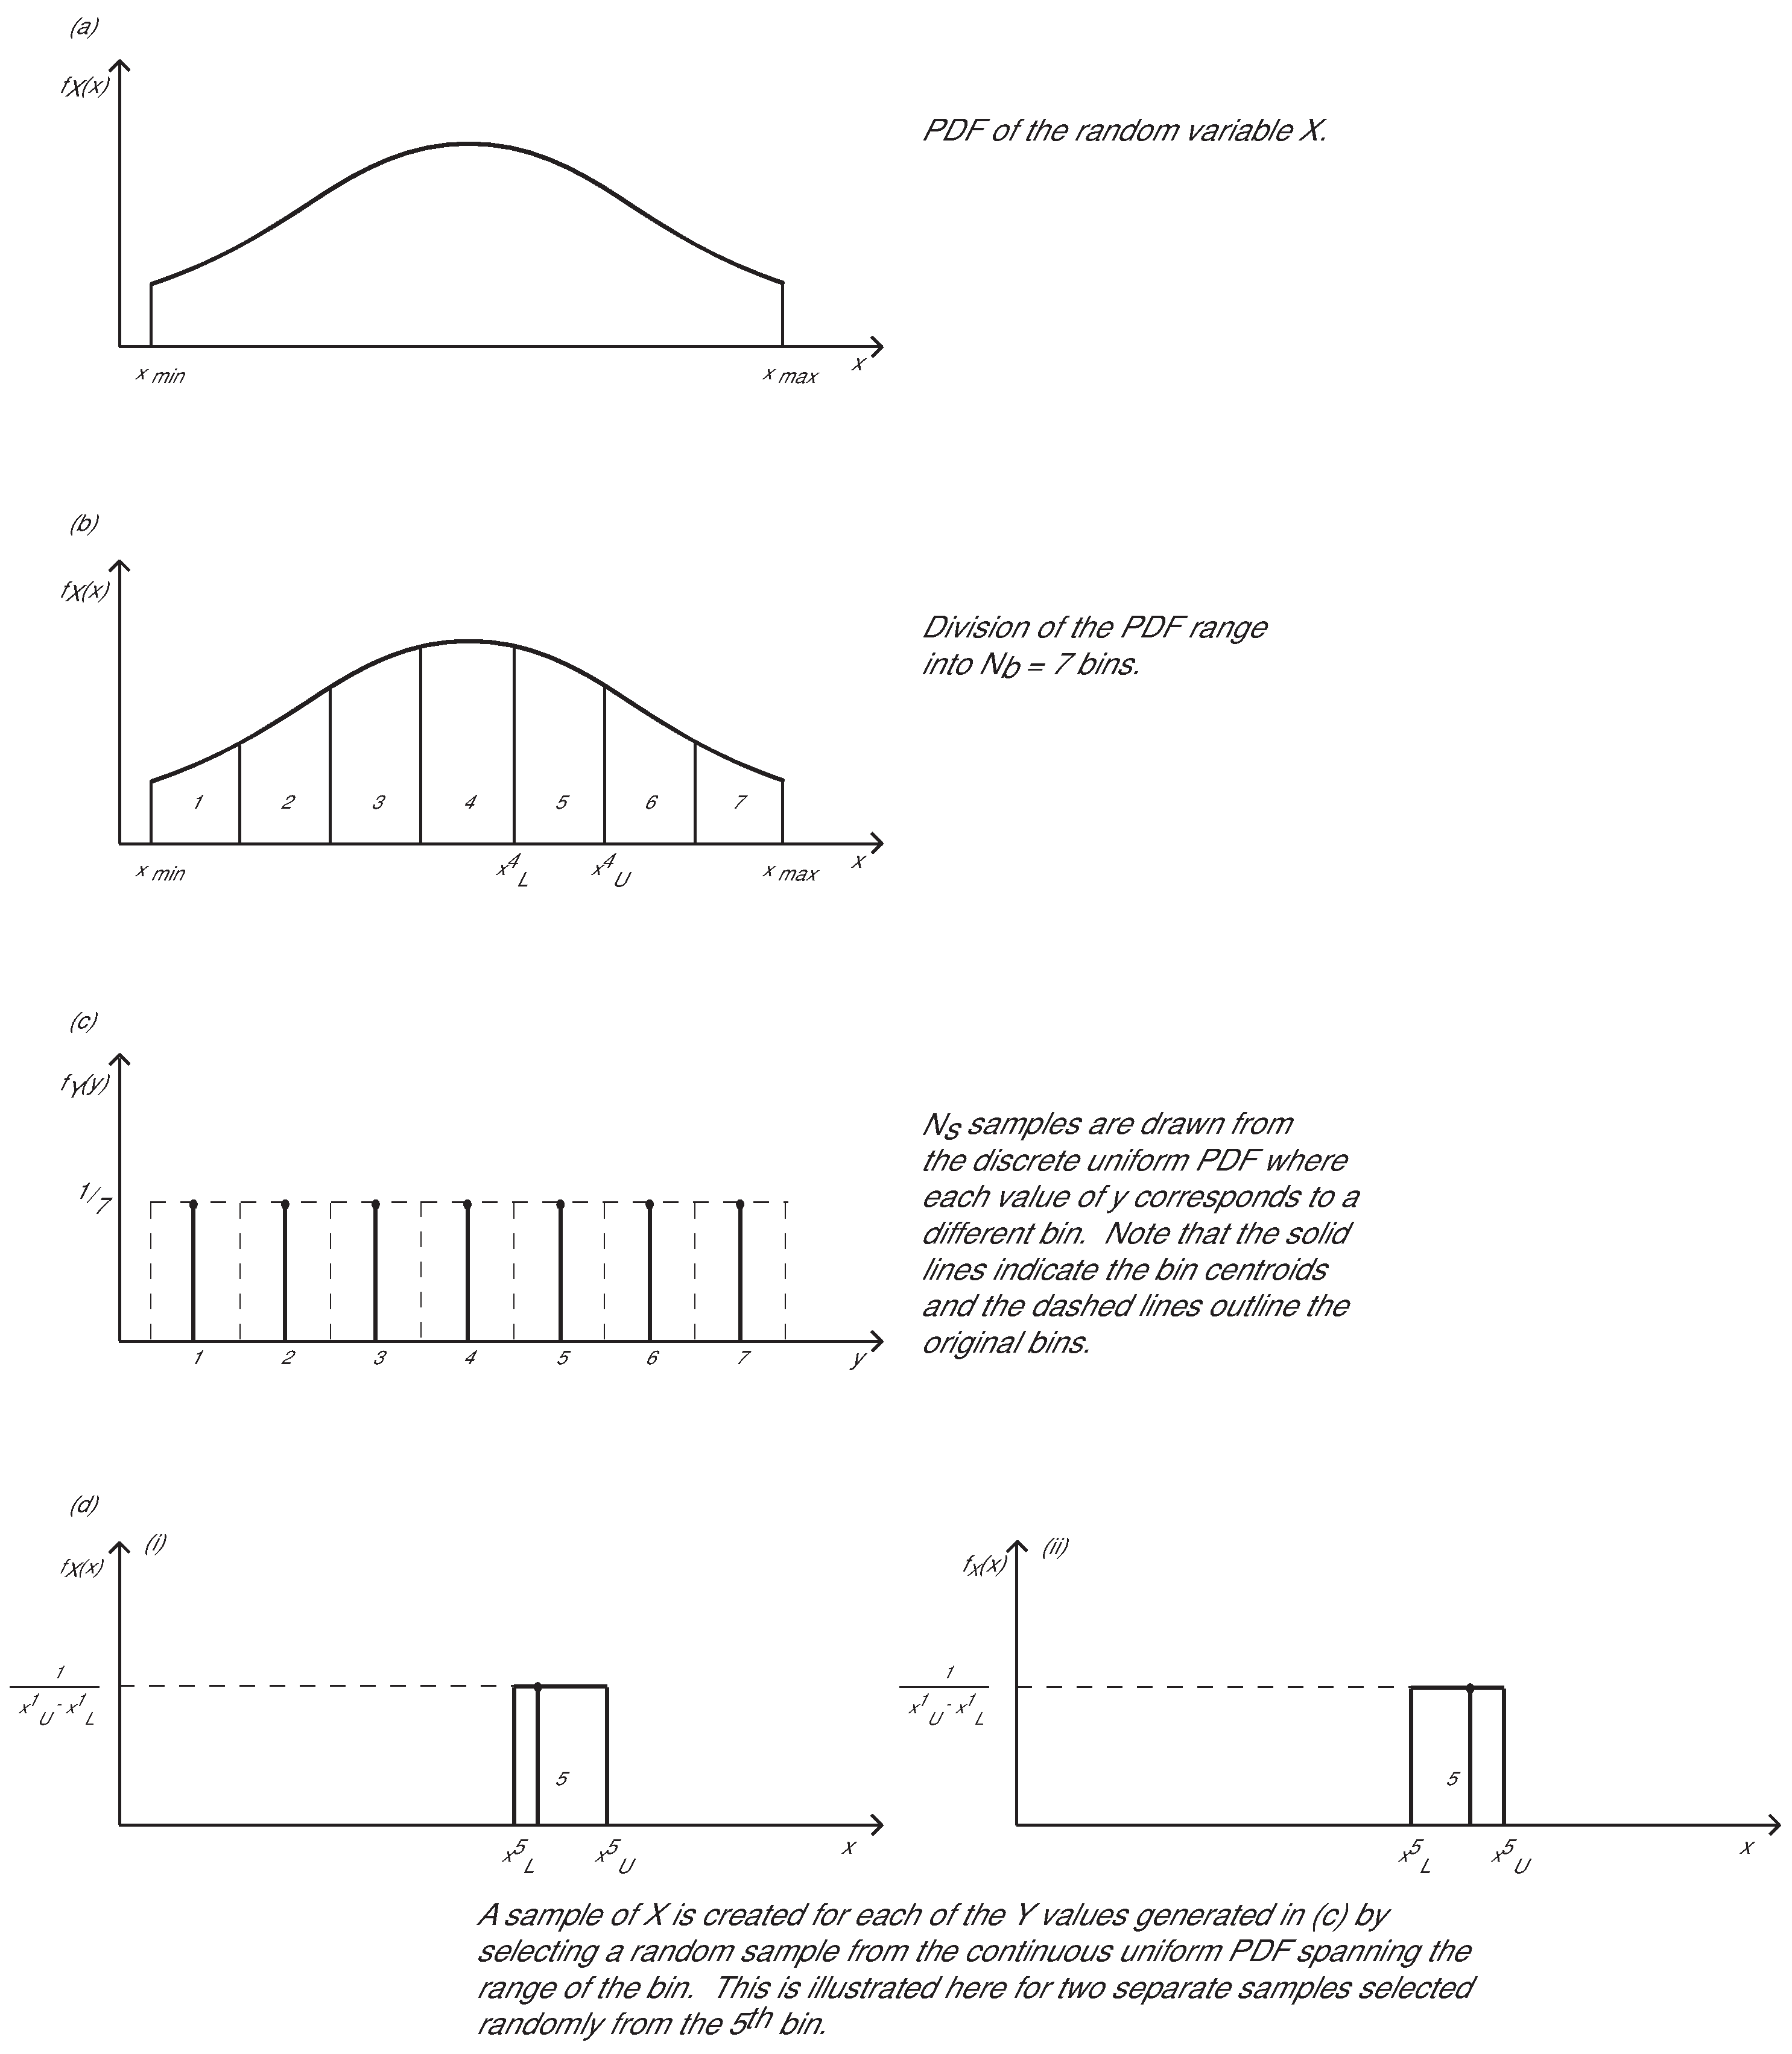
\includegraphics[width=1\textwidth]{fig-hattn-montecarlo}
\caption{Stratified Monte Carlo technique for sampling a PDF. In
this case a normal distribution is shown but any PDF can be used.}
\label{fig-hattn-montecarlo}
\end{figure}

The Probability Density Function (PDF) for the event magnitudes is
based on either the bounded Gutenberg-Richter model \citep{dr_Kramer96a} 
or characteristic earthquake model \citep{eqrm_Schwartz84}. The activity rates of an areal source are computed using the
bounded Gutenberg-Richter earthquake frequency model which is represented by its $A_{min}$ and \emph{b} values (see table \ref{tab:parameters}). 
For fault sources, the magnitude-frequency model is based on either the bounded Gutenberg-Richter or characteristic Earthquake model and 
requires input of the slip rate of the fault by the user for the EQRM to calculate the activity rate. 

The algorithm described in this section is the algorithm applied
to both areal sources and fault sources. While the sampling of the PDF is identical for all models, there are some minor modifications 
where the activity rate is calculated and these differences are discussed below. 

The EQRM application simulates a number $N_s$ of earthquake
events which is unique to each source. Considering the $i^{th}$ source zone (areal source or fault source), the algorithm for
choosing the magnitude of each event can be summarised as follows:

\begin{enumerate}
\item Bound the domain of the PDF with $m_{min}$ and $m_{max}$
(called $x_{min}$ and $x_{max}$ in \fref{fig-hattn-montecarlo}a).

\item Separate the interval $[m_{min}, m_{max}]$ into $N_b$ bins,
and return the bin centroids (\fref{fig-hattn-montecarlo}b).

\item For each of the $N_{s,i}$ events randomly select a bin from
a discrete uniform
  distribution, where $N_{s,i}$ refers to the number of events in the $i^{th}$ source zone.
  This effectively leads to $N_{s,i}/N_b$ earthquakes in
  each magnitude bin and ensures that the full range of magnitudes
  is adequately sampled (\fref{fig-hattn-montecarlo}c).

\item For each of the $N_{s,i}$ events randomly select a magnitude
denoted $r_m$, from a
  continuous uniform distribution that spans the complete range of magnitudes in the
  bin. Note that Step 3 ensures that the entire range of magnitudes is
  adequately sampled whereas this step ensures that all magnitudes can be
  attained (\fref{fig-hattn-montecarlo}d).

\item For each of the $N_{s,i}$ events calculate the event
activity $r_\nu(r_m^*)$, where $r_m^*$ refers to the bin centroid
for the event in question and

\begin{equation}
\label{eq:event-activity} r_\nu(r_m^*) = \frac{N_b}{N_{s,i}}
\times \lambda(A_{min}) \times
P_{GR}(r_m^*-\Delta<R_m<r_m^*+\Delta).
\end{equation}

for Gutenberg-Richter recurrence relationships and

\begin{equation}
\label{eq:event-activity_char} r_\nu(r_m^*) = \frac{N_b}{N_{s,i}}
\times \lambda(A_{min}) \times
P_{CH}(r_m^*-\Delta<R_m<r_m^*+\Delta).
\end{equation}

for Characteristic recrurence relationships (note the $P_{CH}$). The first term in Equation \ref{eq:event-activity} and \ref{eq:event-activity_char}, $\frac{N_b}{N_{s,i}}$,
is the reciprocal of the number of synthetic events in
the bin. This term ensures that the event activity for each
synthetic event scales as the number of generated events is
modified and hence `brings the synthetic results back to the real
world'. The second term in \eref{eq:event-activity},
$\lambda(A_{min})$, represents the number
of earthquakes with magnitude greater than or equal to
$A_{min}$ and is computed differently for each source type (see Sections \ref{sec:rv_areal_GR} and \ref{sec:rv_flt_GR}). $P_{GR}$ and $P_{CH}$ are computed for 
differently for each magnitude-frequency distribution and are outlined in the following sections.

\subsection{Activity rate for areal sources} 
\label{sec:rv_areal_GR}


This is computed by evaluating the bounded Gutenberg-Richter recurrence relationship:

\begin{equation} \label{eq:amin_gr}
\lambda(m) =
A_{min}\frac{e^{-\beta(m-m_{min})}-e^{-\beta(m_{max}-m_{min})}}{1-e^{-\beta(m_{max}-m_{min})}},
\end{equation}

where

\begin{equation}
\beta = b\ln(10).
\end{equation}

The final term in \eref{eq:event-activity} ($P_{GR}$)
represents the actual probability that a real event will fall into
the $r_m^*$ bin in a given year and is computed by evaluating

\begin{equation} \label{eq:P_GR}
P_{GR}(r_m^*-\Delta<R_m<r_m^*+\Delta) =
\frac{f_M(r_m^*)}{\sum\limits_{j=1}^{N_b} f_M(r_{m,j}^*)}
\end{equation}

where $\Delta$ is the half width of the magnitude bins and

\begin{equation} \label{eq:f_m}
f_M(r_m^*) = \frac{\beta
e^{-\beta(r_m^*-m_{min})}}{1-e^{-\beta(m_{max}-m_{min})}},
\end{equation}

%%%%%%%%%%%%%%%%%%%%%%%%%%%%%%%%%%%%%%%%%%%%%%%%%%%%%%%%%%%%%%%%%%%%%%%%%%%%%%%%%%%%%%%%%%

\subsection{Activity rate for faults with bounded Gutenberg Richter model}
\label{sec:rv_flt_GR}
On the basis of equation \ref{eq:amin_gr}, \citet{eqrm_Youngs85} developed a relationship between fault slip 
rate and earthquake recurrence through the use of the total seismic moment rate along a fault ($M_o^T$)which can be found from:

\begin{equation} \label{eq:mot}
\dot{M}_o^T = \mu f_A S
\end{equation}

where $\mu$ is the shear modulus (often taken as 3x10$^{11}$ dyne/cm$^2$), $f_A$ is the fault area and $S$ is the slip rate (cm~/yr). 

We can also find the seismic moment for any earthquake from:

\begin{equation} \label{eq:mo}
M_o = \mu f_A D
\end{equation}

where $D$ is the average displacement along the fault during the earthquake. While equations \ref{eq:mot} and \ref{eq:mo} relate 
seismic moment to geologic data, we can also relate the seismic moment to earthquake magnitude from theoretical considerations and 
empirical observations by:

\begin{equation} \label{eq:mo_mag}
M_o = 10^{cm+d}
\end{equation}

where $c=1.5$ and $d=16.1$ from \citet{eqrm_Hanks79}. \citet{eqrm_Youngs85} then showed that seismic 
moment rate can be linked to the earthquake recurrence rate by:

\begin{equation} \label{eq:mot_int}
\dot{M}_o^T = \int_{m_{min}}^{m_{max}} \; f(m) \; M_o(m) \; dm
\end{equation}

where $f(m)$ is the probability density function (PDF) of the earthquake recurrence rate from equation \ref{eq:f_m} and figure \ref{fig:pdf}. 
By using equations \ref{eq:mot} and \ref{eq:mo}, we can rewrite equation \ref{eq:mot_int} as:

\begin{equation} \label{eq:lam_exp1}
\mu f_A S= \frac{ b \lambda _{m_{min}} M_o^{max} e^{- \beta (m_{max} - m_{min} )} }  { (c - b) (1-e^{-\beta (m_{max} - m_{min}) })  }
\end{equation}

where M$_o^{max}$ is the seismic moment of m$_{max}$ which can be found from equation \ref{eq:mo_mag}. Equation \ref{eq:lam_exp1} 
can be rearranged to find the activity rate above the minimum magnitude ($\lambda m_{min}$) :

\begin{equation} \label{eq:lam_exp}
\lambda m_{min} = \frac{ \mu f_A S (c - b) (1-e^{-\beta (m_{max} - m_{min}) }) } { M_o^{max}  e^{- \beta (m_{max} - m_{min} )} }
\end{equation}

In practical applications, the $b$-value can be obtained from historical seismicity in a box bounding the 
fault \citep{eqrm_Schwartz84,eqrm_Youngs85} or if there is insufficient historical records near the fault, 
then it can be approximated by the $b$-value of the source zone that the fault lies within. 

To calculate $P_{GR}$, equation \ref{eq:P_GR} and \label{eq:f_m} can be used. 

%%%%%%%%%%%%%%%%%%%%%%%%%%%%%%%%%%%%%%%%%%%%%%%%%%%%%%%%%%%%%%%%%%%%%%%%%%%%%%%%%%%%%%%%%%
\subsection{Activity rate for faults with bounded Characteristic Earthquake model} 
\label{sec:rv_flt_ch}

Following the same approach as in equations \ref{eq:lam_exp1} and  \ref{eq:lam_exp}, and using the shape of the characteristic 
earthquake density function in figure \ref{fig:pdf} we can relate the activity rate to the slip rate. To find the activity 
rate ($\lambda m$) we require the slip rate ($S$), $b$ value, and $m_{max}$ for the fault. We can then use 
a 3 step process where first we solve for the non-characteristic or exponential part of the distribution ($\lambda m_{min} - \lambda m_{c}$):

\begin{equation} \label{eq:lam_0}
\lambda (m_{min} - m_{c}) = \frac { \mu f_A S (1-e ^{- \beta (m_{max} - m_{min} - 0.5)}) } { M_o^{max} K e ^{- \beta (m_{max} - m_{min} - 0.5)  }  }
\end{equation}

where $K$ is equal to:
\begin{equation}
K = \frac { b 10 ^ {-c/2} }  { c- b } + \frac { b e ^{\beta} (1 - 10^{-c/2})  }  {  c } .
\end{equation}

Now we can find  the activity rate for the characteristic part of the distribution ($\lambda m_{c}$) which defines the cumulative number of earthquakes greater than $m_c$,  :

\begin{equation} \label{eq:lam_c}
\lambda m_c = \frac { \beta (\lambda m_{min} - \lambda m_{c}) e ^{-\beta ( m_{max} - m_{min} - 1.5)} }  { 2 ( 1 -  e ^{- \beta (m_{max} - m_{min} - 0.5)  }) }
\end{equation}

and using the results from equations \ref{eq:lam_0} and \ref{eq:lam_c} we can find the cumulative activity rate above the minimum magnitude ($\lambda m_{min}$) from:
\begin{equation} \label{eq:lam_ch}
\lambda m_{min} = (\lambda (m_{min} - m_{c})) + \lambda m_{c}
\end{equation}

\begin{figure}[htp]
\centerline{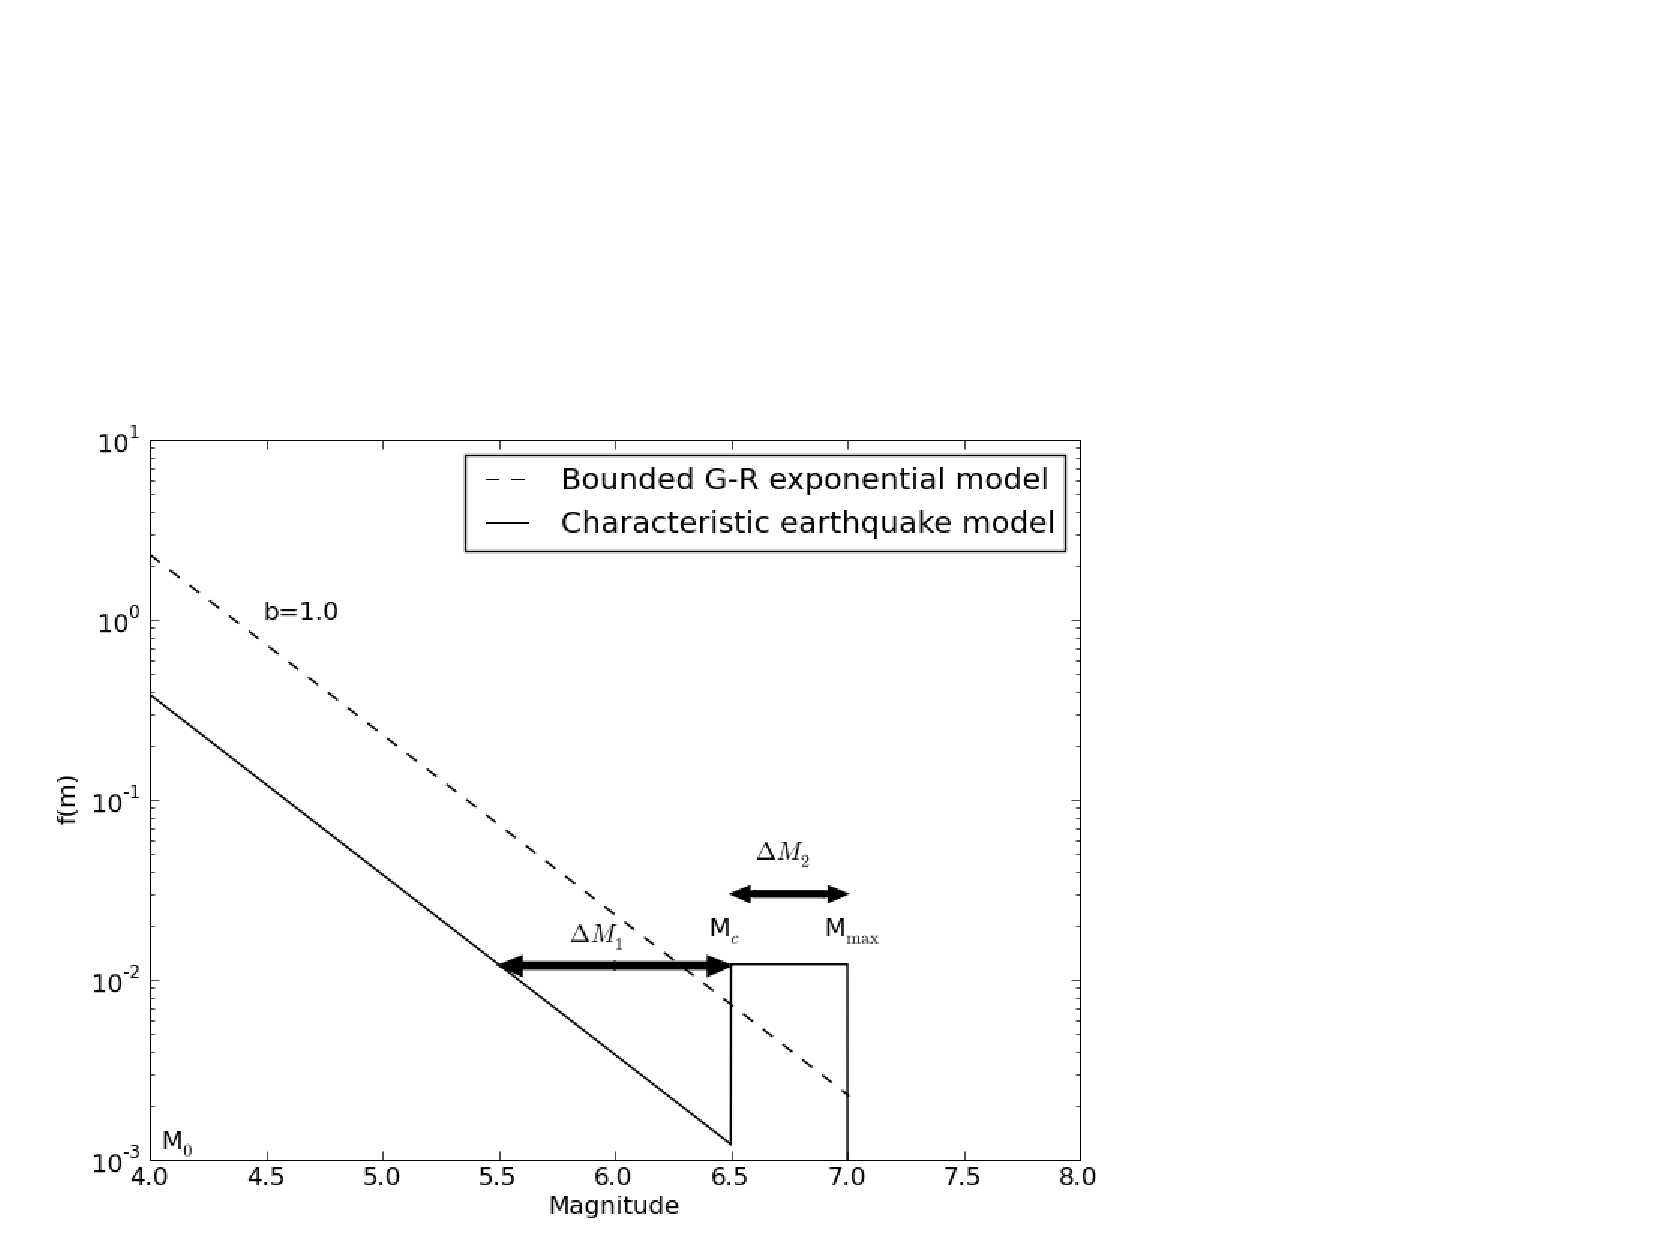
\includegraphics[width=12cm]{fig-hsource-pdf_ch}}
\caption{The magnitude-frequency relationship for the bounded G-R exponential model (equation \ref{eq:f_m}) and the characteristic earthquake model (equation \ref{eq:pdf_ch}).}
\label{fig:pdf}
\end{figure}

The final term in \eref{eq:event-activity}
represents the actual probability that a real event will fall into
the $r_m^*$ bin in a given year and is computed by evaluating

\begin{equation} \label{eq:P_CH}
P_{CH}(r_m^*-\Delta<R_m<r_m^*+\Delta) =
\frac{f_M(r_m^*)}{\sum\limits_{j=1}^{N_b} f_M(r_{m,j}^*)}
\end{equation}

where

\begin{equation} \label{eq:pdf_ch}
f_M(r_m^*) = \left\{
\begin{array}{ll}
0 & \quad \mbox{for $m < m_{min}$} \\
\frac{\beta e ^{- \beta (m-m_{min})}}{1-e^{-\beta (m_{max} - m_{min} - \Delta m_{2})}} \frac{1}{1+C}& \quad \mbox{for $m_{min} \leq m \leq m_{c} = m_{max} - \Delta m_{2}$} \\
\frac{\beta e ^{- \beta (m_{max}-m_{min}-\Delta m_{1} - \Delta m_{2})}}{1-e^{-\beta (m_{max} - m_{min} - \Delta m_{2})}}  \frac{1}{1+C}& \quad \mbox{for $m_{c} = m_{max} - \Delta m_{2} \leq m \leq m_{max}$} \\
0 & \quad \mbox{for $m > m_{max}$} \\ 
\end{array}
 \right. 
\end{equation}

for the Characteristic Earthquake model\citep{eqrm_Schwartz84}, where the constant C is given by:

\begin{equation}
C = \frac{\beta e ^{- \beta (m_{max}-m_{min}-\Delta m_{1} - \Delta m_{2})}}  {1-e^{-\beta (m_{max} - m_{min} - \Delta m_{2})}}  \Delta m_{2} .
\end{equation}


\citep{dr_Kramer96a}. Note that $r_\nu$ represents the frequency of occurence in terms
of a number per year and can be thought of as the synthetic
version of the activity rate ($\lambda$) for the simulated event catalogue.
\end{enumerate}

\subsection{Event Magnitude Examples} 
\label{sec:ev_mag_example}

Figures \ref{fig:source-catalogue-results1}a to \ref{fig:source-catalogue-results4}a
illustrate histograms of the event magnitudes simulated for three
different source zone combinations. Note that the fifteen bars in
Figures \ref{fig:source-catalogue-results1}a to \ref{fig:source-catalogue-results4}a
correspond to the fifteen different magnitude bins. The event
activity $r_v$ for the same source zone combinations are shown in
Figures \ref{fig:source-catalogue-results1}c to \ref{fig:source-catalogue-results4}c.

\begin{figure}
  \vspace{0.8em}
\begin{center}
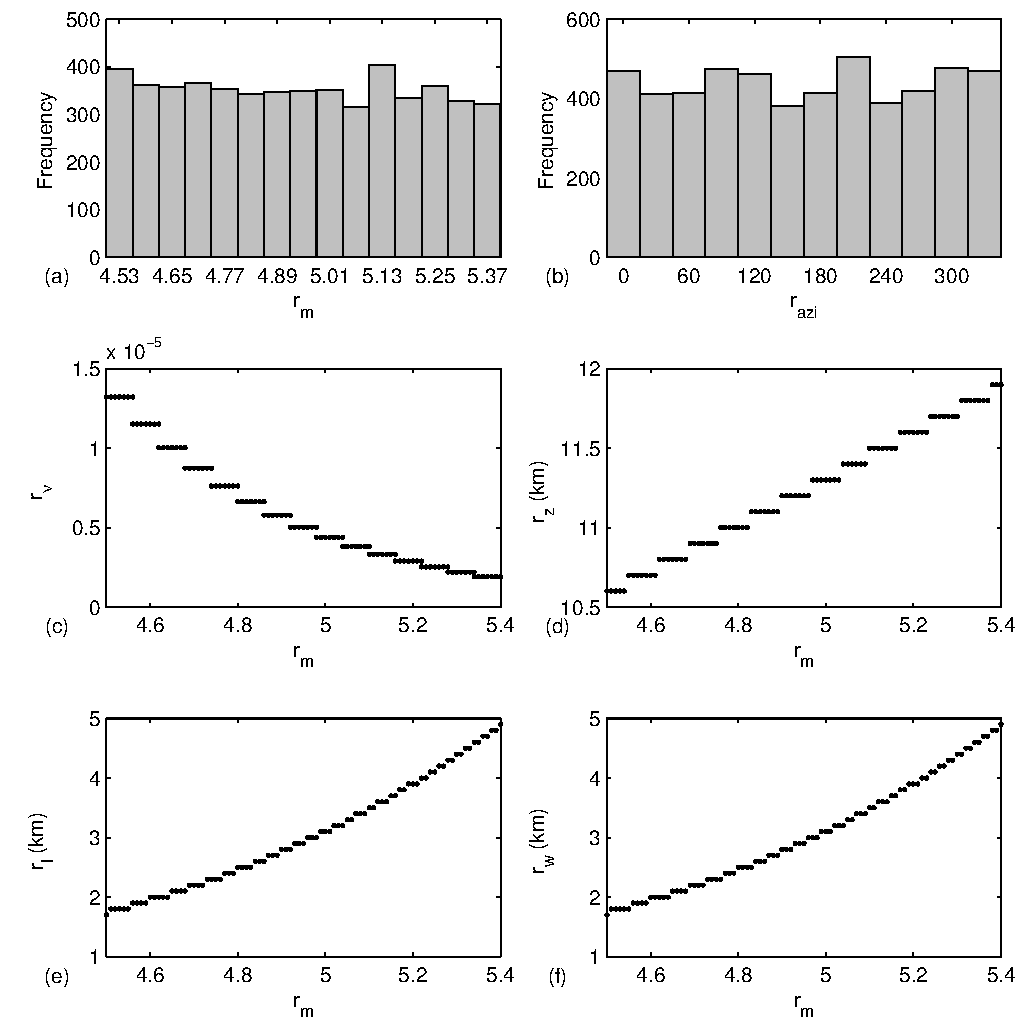
\includegraphics[width=1\textwidth]{fig-hsource-eventstatstri}
\end{center}
\caption{Simulated events for the Newcastle Triangle Zone (see
\citealt{dr_Dhu02b}). Plots (a) and (b) show histograms of the
rupture magnitude $r_m$ and rupture azimuth $r_{azi}$
respectively. Plots (c), (d), (e) and (f) illustrate the
relationship between the event magnitude $r_m$ and the event
activity $r_\nu$, the depth to the rupture centroid $r_z$, the
length of the rupture $r_l$ and the width of the rupture $r_w$
respectively. The number of events was
$5000$.} \label{fig:source-catalogue-results1}
\end{figure}

\begin{figure}
\begin{center}
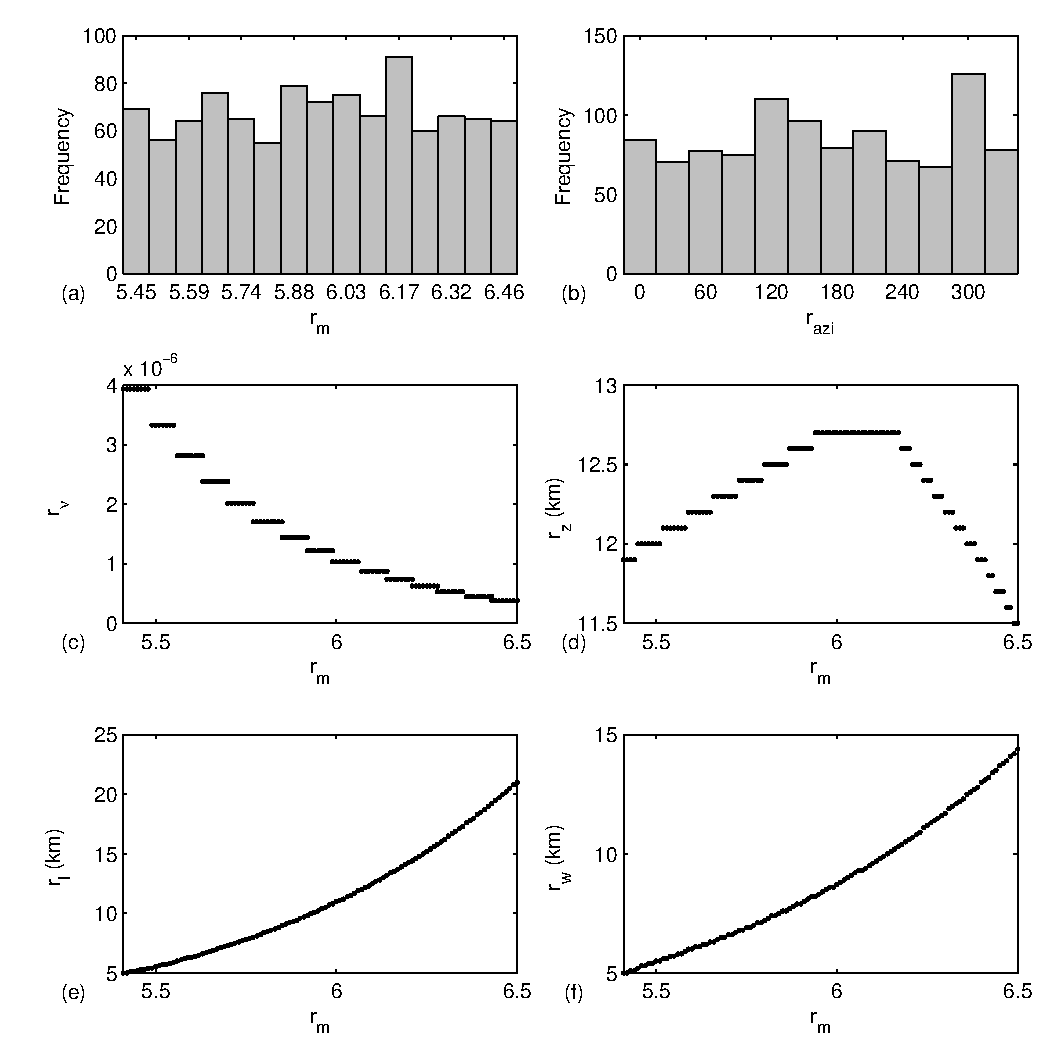
\includegraphics[width=1\textwidth]{fig-hsource-eventstatsrec}
\end{center}
\caption{Simulated events for the Newcastle Rectangle Zone (see
\citealt{dr_Dhu02b}). Parts (a) to (f) are the same as those
described in \fref{fig:source-catalogue-results1}. The number of events was $3000$.}
\label{fig:source-catalogue-results2}
\end{figure}

\begin{figure}
\begin{center}
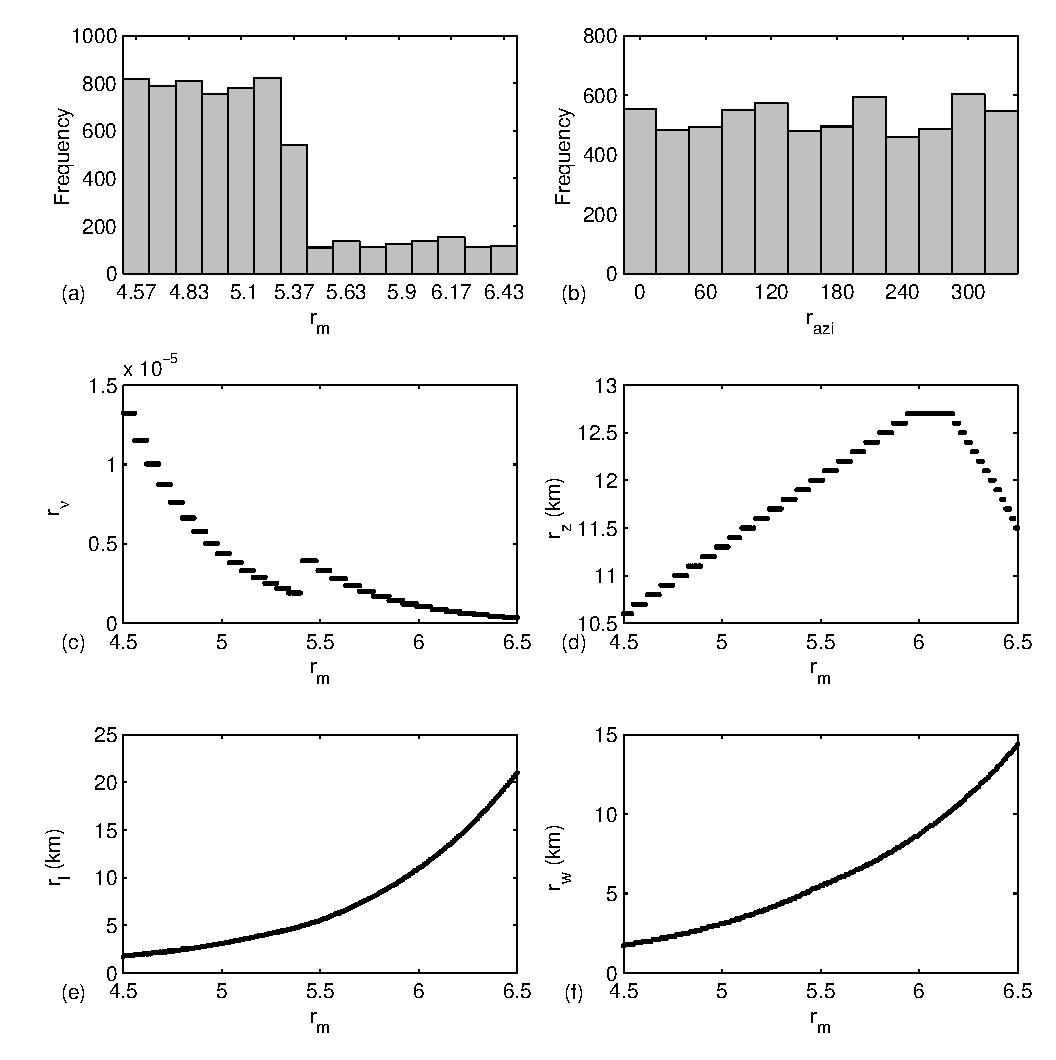
\includegraphics[width=1\textwidth]{fig-hsource-eventstats_tri_rec}
\end{center}
 \caption{Simulated
events when the Newcastle Triangle Zone and Newcastle Fault Zone
are considered together (see \citealt{dr_Dhu02b}). Parts (a) to
(f) are the same as those described in
\fref{fig:source-catalogue-results1}. The number of events
was 5000 and 3000, where the source zones
$1$ and $2$ refer to the the Newcastle Triangle Zone (NTZ) and the
Newcastle Fault Zone respectively.}
\label{fig:source-catalogue-results3}
\end{figure}



\begin{figure}
\begin{center}
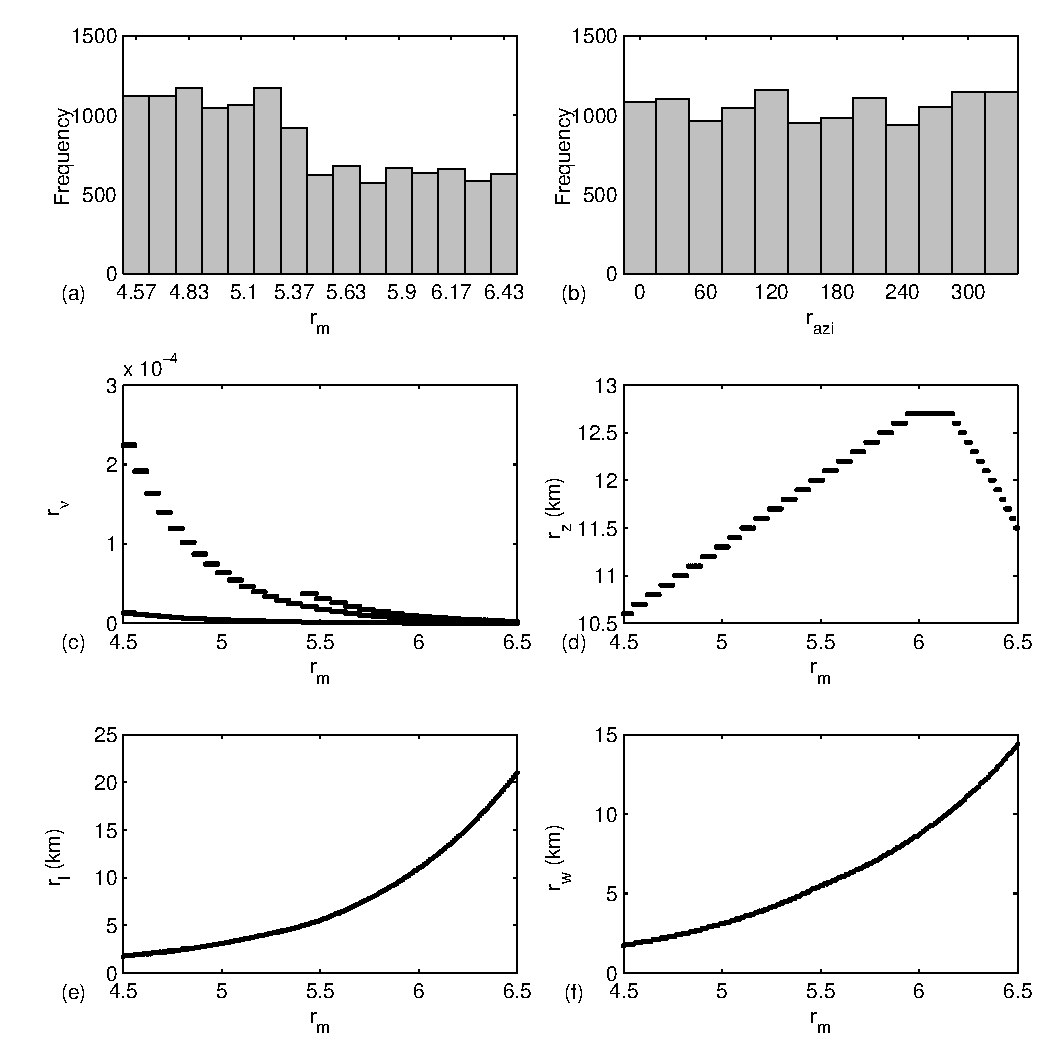
\includegraphics[width=1\textwidth]{fig-hsource-eventstatsall}
\end{center}
\caption{Simulated events for all six of the source zones used in
the Newcastle and Lake Macquarie study (see \citealt{dr_Dhu02b}).
Parts (a) to (f) are the same as those described in
\fref{fig:source-catalogue-results1}. The desired number of events
was defined by $ntrgvector = [5000,1000,1000,3000,1000,1000]$
where the source zones $1$ to $6$ refer to the the Newcastle
Triangle Zone (NTZ) the Tasman Sea Margin Zone Subset 1 (TSMZ1),
the TSMZ2, the Newcastle Fault Zone, the TSMZ3 and the TSMZ4
respectively.} \label{fig:source-catalogue-results4}
\end{figure}



\section{Generating synthetic earthquakes in areal source zones}
\label{sec:areal_gen}

This section describes the procedure for generating synthetic earthquakes in areal source zones that are considered background seismicity, such that they can be located
anywhere in the source polygon. Later we will outline the method for generating earthquakes on pre-defined fault sources. 

The location of each event centroid is assigned randomly within an areal source zone. 
This assignment is done in such a way that the event centroid has
an equal probability of being located anywhere in the source
polygon. 


\subsection{Dimensions and position of the rupture plane}
\label{sec:dim-rupture}

The width and length of the rupture and position of the rupture
centroid are computed using empirical
rules based on the moment magnitude ($r_m$) of the event. In the current version of the EQRM, three scaling 
rules are available for use; 
\begin{itemize}
\item The \citet{eqrm_Wells94} emperical relationships, 
\item A modified version of \citet{eqrm_Wells94} presented by Mendez, 2002 ([$\textit{pers. comm.}$]), and; 
\item Scaling laws for stable continental regions developed by \citet{eqrm_Leonard10}.
\end{itemize}

The location of the rupture plane
is constrained to lie within a virtual fault
which is described by the depth to its top (equivalent to the
depth to the seismogenic region ($f_z$), see
table \ref{tab:parameters}), its length ($f_l$), its width
($f_w$) and its dip ($r_{dip}$). Note that by definition the dip of the
 rupture plane is the same as the dip of the virtual fault. 

\subsubsection{\citep{eqrm_Wells94} Scaling Laws}

This scaling law has gained significant popularity for determining rupture dimensions and displacement for crustal earthquakes. The EQRM calculates the dimensions by first 
constraining the rupture area ($r_A$) for different fault types:

\begin{equation} \label{ra}
r_A = 
\begin{cases}
10^{-2.87 + 0.82r_m}	& \quad \mbox{if \texttt{fault type $=$  normal}} \\
10^{-3.99 + 0.98r_m}	& \quad \mbox{if \texttt{fault type $=$  reverse}} \\
10^{-3.42 + 0.90r_m}	& \quad \mbox{if \texttt{fault type $=$  strike slip}} \\
10^{-3.497 + 0.91r_m}	& \quad \mbox{if \texttt{fault type $=$  unspecified}} . \\
\end{cases}
\end{equation}

where $r_m$ is the moment magnitude of the rupture event determined in section \ref{sec:magnitude_selection}. 

Next the rupture width ($r_w$, in km) is computed with a restriction to stop the rupture from extending 
outside the seismogenic zone defined by $f_z^{top}$ to $f_z^{bot}$. The calculation of the rupture width is a two stage process:


\begin{equation}\label{rw}
r_w^{WC} = 
\begin{cases}
10^{-1.14 + 0.35r_m}	& \quad \mbox{if \texttt{fault type $=$  normal}} \\
10^{-1.61 + 0.41r_m}	& \quad \mbox{if \texttt{fault type $=$  reverse}} \\
10^{-0.76 + 0.27r_m}	& \quad \mbox{if \texttt{fault type $=$  strike slip}} \\
10^{-1.01 + 0.32r_m}	& \quad \mbox{if \texttt{fault type $=$  unspecified}} \\
\end{cases}
\end{equation}


\begin{equation} \label{eq:rw}
r_w = \mathbf{min}\{r_w^{WC}, f_w\} .
\end{equation}

The rupture length ($r_l$) is calculated as follows, making sure it does not extend beyond the fault length ($f_l$) from:

\begin{equation}
r_l = \mathbf{min}\left\{\frac{r_A}{r_w}, f_l\right\} .
\end{equation}


\subsubsection{Modified \citep{eqrm_Wells94} Scaling Laws}

Firstly, the area of the rupture plane $r_A$ is defined as
\begin{equation}
r_A = 10^{r_m - 4.02}
\end{equation}
which represents a subtle change from that defined by
\citep{eqrm_Wells94}. Empirical relationships for the width ($r_w$)
and length ($r_l$) of the rupture plane were defined by Mendez (2002
[\textit{pers. comm.}]). The width is defined in a two step
process as follows

\begin{equation}
 f_1 = \left \{ \begin{array}{ll}
 1 & \textrm{if $r_m \leq 5.5$} \\
\frac{1}{\sqrt[\leftroot{-2}\uproot{2}4]{1+2(r_m-5.5)\sin(r_{dip})}} & \textrm{if $r_m>5.5$} \\
\end{array} \right.
\end{equation}

and

\begin{equation}
r_w = \textrm{min$\{f_1\sqrt{r_A},f_w\}$}.
\end{equation}

\subsubsection{Leonard (2010) Stable Continental Regions Scaling Law}
This scaling law is recommended for all intraplate settings. First the rupture area ($r_A$) is calculated from the magnitude ($r_m$) by:

\begin{equation}
r_{A} = 10^{r_m-4.1833}
\end{equation}

Next the rupture length ($r_l$) is calculated from:

\begin{equation}\label{leonard_rw}
r_w = 
\begin{cases}
10^{0.6r_m-2.59}	& \quad \mbox{if \texttt{$M_w$ < 4.975}} \\
10^{0.5r_m-2.095}	& \quad \mbox{if \texttt{$M_w$ $\ge$ 4.975}} \\
\end{cases}
\end{equation}

and then it is a trivial step to find the rupture width ($r_l$).

\subsection{Azimuth and dip of rupture}
\label{sec:az-dip-rupture}

The rupture azimuth of each event may be forced to lie within a
user defined range
\begin{center} $\phi - \Delta_{\phi} \leq r_\phi \leq \phi + \Delta_{\phi}$ \end{center}
where $\phi$ and $\Delta_{\phi}$ are the azimuth and azimuth sampling range respectively. The
default values for $\phi$ and $\Delta_{\phi}$ are $180^o$ and $180^o$
respectively. 

The dip of the rupture ($r_{dip}$), and a sampling range ($\Delta_{dip}$) are assigned by the 
user for each areal source zone. The dip of the rupture trace is measured from the
ground surface and the direction of dip is such that the plane is
located in the region of $y>0$ in the local coordinate system.
Note that sampling across a dip range will impact the attenuation models in a variety of ways (see \sref{ch:atten}). 
For example, when using an attenuation model that depends 
on the Joyner-Boore distance, the practical effect of a change in dip can be compensated by a
horizontal translation of the rupture trace. In such cases the random
location of the rupture trace negates the need to select the dip randomly.

\subsection{Location of synthetic events in areal sources}
\label{sec:areal_locn}

The first phase of locating the events involves positioning the
centre point of each rupture trace ($r_c^{lat}$,$r_c^{lon}$). A
rectangular box is generated over the top of the source zone polygon. The
box is bounded by the minimum and maximum latitude and the
minimum and maximum longitude of the source zone itself. 

% Need to change this to have no underlying grid. 
% \begin{figure}
% \begin{center}
% 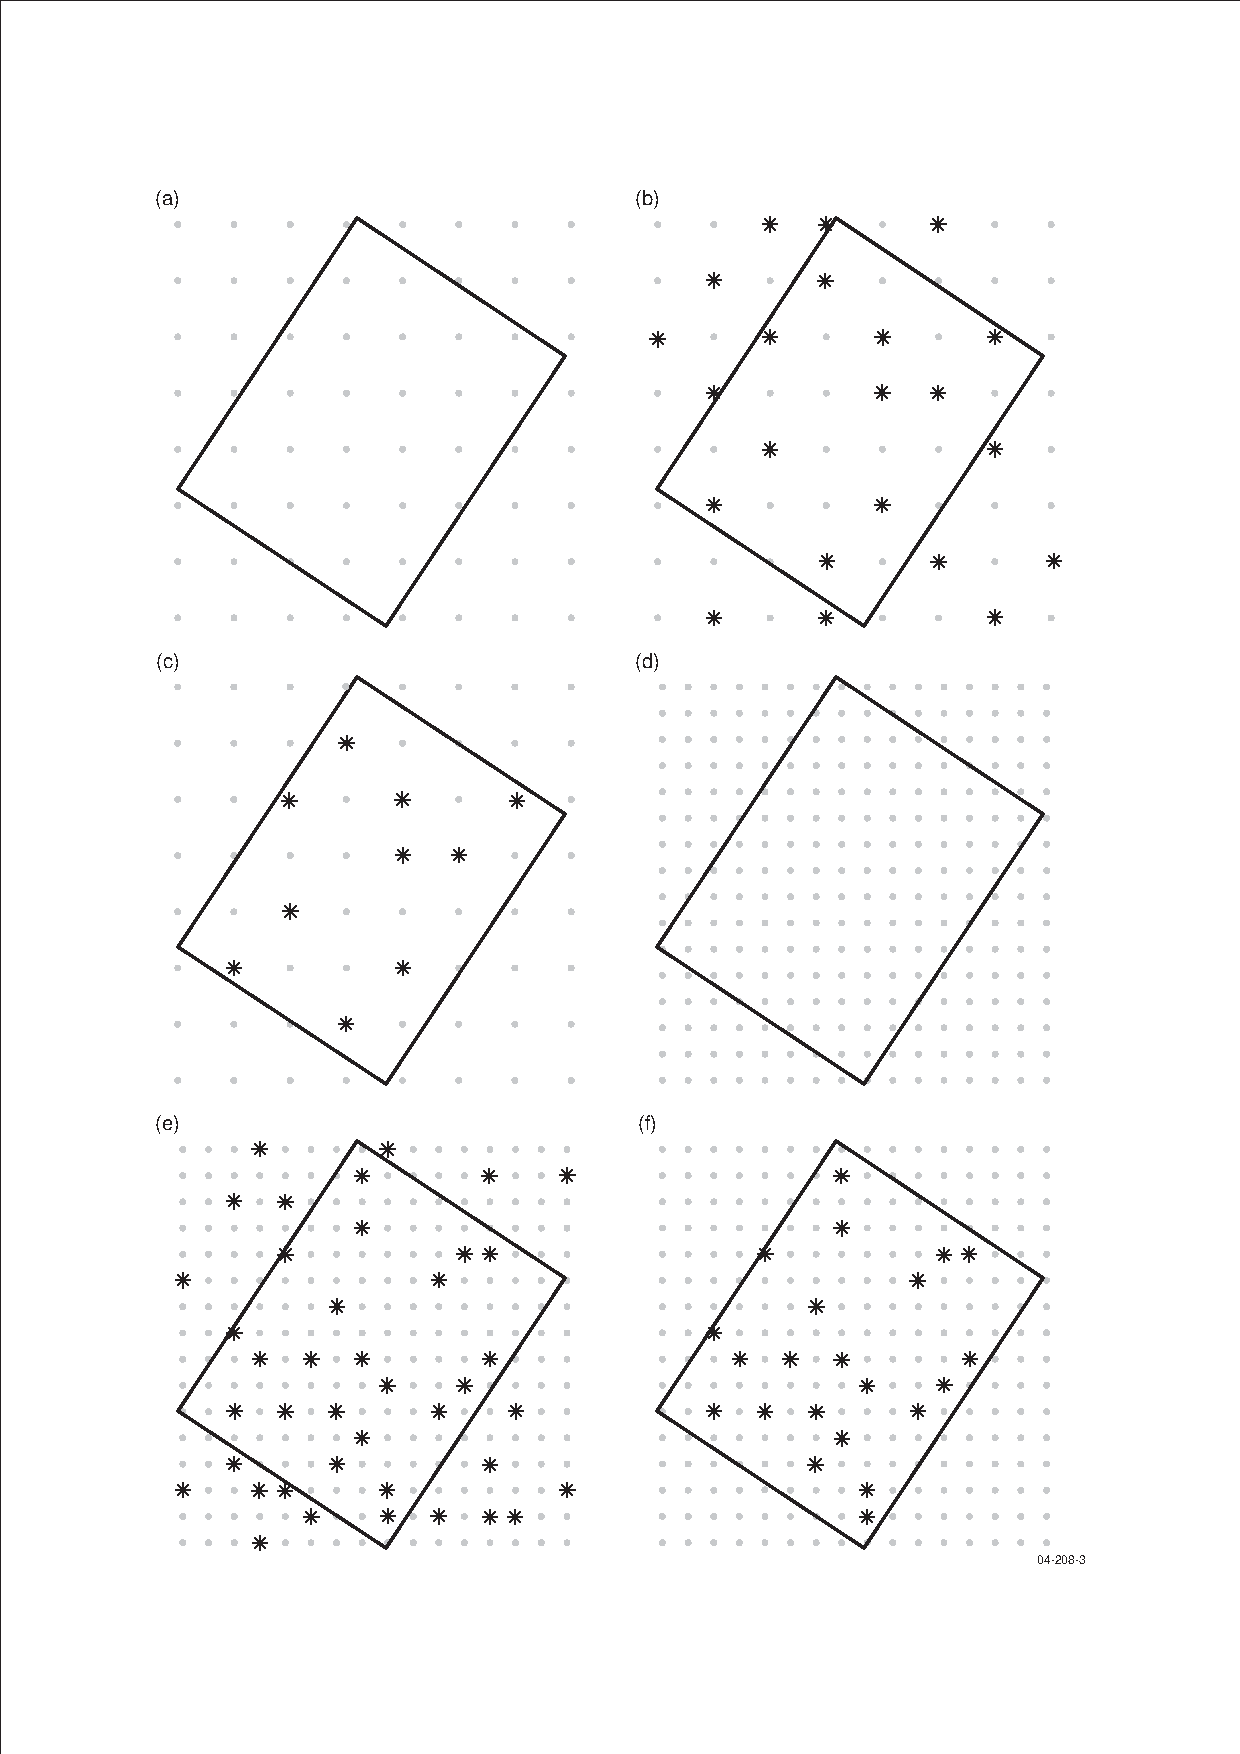
\includegraphics[width=0.9\textwidth]{fig-hsource-trace-starts}
% \end{center}
% \caption{Random selection of rupture centroids for a
% rectangular `generation polygon'. (a) to (c) illustrate the first
% iteration and (d) to (f) the second iteration after contraction of
% the grid spacing.} \label{fig:source-trace-starts}
% \end{figure}

The rupture centroid of each event is then randomly placed within the box 
using a discrete uniform probability density function. The individual event is then checked to identify whether 
it falls within the source polygon or not. Events that fall within the source polygon 
are kept and those that lie outside it are discarded. This process continues until the number of events 
defined by the user for the source zone is reached.

The second phase of locating events involves positioning the start and end
point of the rupture trace. Assume for the moment that both the
length and azimuth of the rupture trace are already known (see
\sref{sec:dim-rupture} and \sref{sec:az-dip-rupture} respectively
for a description of how these are computed). It is then a trivial
process to compute the start and end of the rupture trace
$(r_s^{lat},r_s^{lon}$ and $r_e^{lat},r_e^{lon})$. It is important to note that the EQRM will allow the 
start or end points of the rupture trace to lie outside of the source polygon 
providing the rupture centroid is located within the polygon. Therefore the source zone polygon 
is only used to constrain the rupture centroid ($r_c^{lat},r_c^{lon}$).

The next step involves determining the rupture centroid location.
Recall from \sref{sec:source-EQcat} that the rupture centroid
$(r_x,r_y,r_z)$ is defined in terms of a local coordinate system.
The depth of the rupture centroid is determined in a two step
process as follows:

\begin{equation}
r_z = \textrm{min$\{f_z+\frac{f_2}{3}f_w\sin(r_{dip}),
f_z+f_w\sin(r_{dip})-\frac{1}{2}r_w\sin(r_{dip})\}$}
\end{equation}

where

\begin{equation}
f_2 = \left \{ \begin{array}{ll} 1 & \textrm{if $r_m\leq4$} \\
1 + \frac{r_m-4}{2} & \textrm{if $4<r_m\leq6$} \\
2 & \textrm{if $r_m\geq6$} \\
\end{array} \right.
\end{equation}



The other two coordinates of the rupture centroid are given by
\begin{equation}
r_y = r_z\cot(r_{dip})
\end{equation}

and

\begin{equation}
r_x = \frac{r_l}{2}.
\end{equation}


The depth to the rupture centroid $r_z$ and the length and width
of the rupture plane are illustrated for four separate simulations
in Figures \ref{fig:source-catalogue-results1} to \ref{fig:source-catalogue-results4}(d),
(e) and (f) respectively.

\subsection{Overlapping source zones}

The concept of overlapping zones in a source model is useful for
accommodating background seismicity. In principle, the code can
accommodate overlapping seismic zones, i.e. where two seismic
zones share a common geographical region. However, it should be
noted that earthquakes will be distributed randomly in the common
region for each zone that exists. That is, a simulation using
overlapping source zones (such as that shown in
\fref{fig:h-source-overlapping}(a)) may lead to a greater number
of simulated earthquake\index{simulated earthquake}s in the common
region than may be warranted by the source model. This only poses
a problem if the recurrence relationship (i.e. the $a$, $b$
parameters) being used has not been modified to account for the
`double counting' in the simulated catalogue (generally this will
not have been done). To overcome this problem, it is advisable to
define the source zones in such a way that there are no
overlapping regions. \fref{fig:h-source-overlapping} demonstrates
two different techniques that can be used to incorporate
overlapping source zones in the EQRM. Both of the illustrated
techniques are based on creating a doughnut.

\begin{figure}[htp]
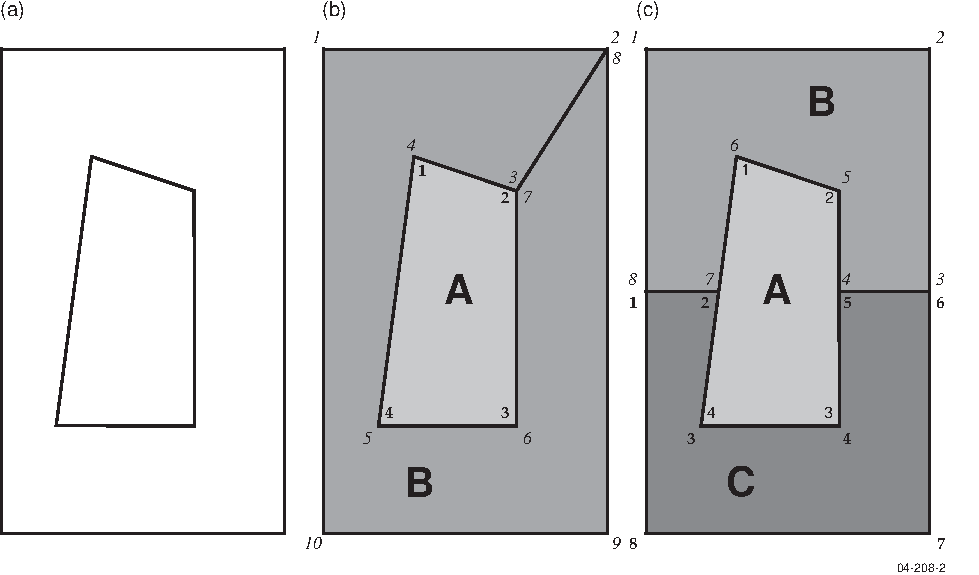
\includegraphics[width=1\textwidth]{fig-hsource-overlapping-zones}
\caption{Overlapping source zones shown in (a) can be incorporated
into the EQRM by cutting out a doughnut (b) or splitting the outer
polygon (c). The numbers in different fonts illustrate how the
polygon vertices could be listed in the input file.
} \label{fig:h-source-overlapping}
\end{figure}



% \subsection{Using multiple source zones - Incorporating epistemic uncertainty}
% \label{sec:source-multizones}

% Recall that \sref{sec:source-EQcat} introduced two techniques for
% passing source models to the EQRM:
% \begin{enumerate}
% \item the
% \typeparfilecaption{<site\_loc>}{\_par}{\_sourcezones}{.txt} and
% \typeparfile{<site\_loc>}{\_par\_sou}{rcepolys}{.txt} file pair,
% and \item the
% \typeparfilecaption{<site\_loc>}{\_par}{\_source}{.mat} file.
% \end{enumerate}
% Recall also that the notion of a `generation
% polygon'\index{generation polygon} was introduced where the
% generation polygons are simply the individual source zones when
% Technique 1 is used, and `generation polygon' refers to the
% polygons in the \typevar{gen}{erat}{ion} variable when Technique 2
% is used. This definition ensured that the discussion of earthquake
% location (\sref{sec:rup-location}), rupture geometry
% (\sref{sec:dim-rupture}), azimuth and dip
% (\sref{sec:az-dip-rupture}) described above is applicable to both
% of the two techniques for providing source information to the
% EQRM. When Technique 2 is used, however, a minor modification must
% be made to the algorithm described for magnitude and event
% activity determination (see \sref{sec:magnitude_selection}). To
% explain the differences in the algorithm and to explain the
% incorporation of multiple source zone models (epistemic
% uncertainty with source models) the reader will need to understand
% the contents of the
% \typeparfile{<site\_loc>}{\_par}{\_source}{.mat} file.

% The \typeparfile{<site\_loc>}{\_par}{\_source}{.mat} file contains
% the following two variables:
% \begin{enumerate}
% \item The \typevar{gen}{erat}{ion} variable is a MATLAB structure
% containing the fields \texttt{zones} and \texttt{polys}. The field
% \texttt{zones} is a matrix containing the same format as that
% described in \tref{tab:site-loc-par-sourcezones}. The number of
% rows refers to the number of `generation polygons' to be used in
% the generation process. It is common to have 2 `generation
% polygons' arranged in a doughnut shape with an inner and outer
% polygon. The inner polygon is typically centered on the region of
% interest and can be used to simulate a larger number of
% earthquakes (hence higher spatial concentration) than the outer
% polygon. The field \texttt{polys} is a matrix using the same
% format as \tref{tab:site-loc-par-sourcepolys} to describe the
% vertices of the polygons in the field \texttt{zones}. \item The
% \typevar{sou}{rc}{e} variable is a MATLAB structure array
% containing one element for each source zone model to be used. The
% number of elements in the \typevar{sou}{rc}{e} structure array
% corresponds to the number of source zone models to be used in the
% simulation. Each element has fields \texttt{zones}, \texttt{polys}
% and \texttt{weight}. The fields \texttt{zones} and \texttt{polys}
% are similar to those described in 1 above, however this time they
% represent the individual source source zones for the source model.
% The field \texttt{weight} represents the weight to be applied to
% the source zone model.
% \end{enumerate}

% When using Technique 2 the \typevar{gen}{er}{ation} is used to
% define the `generation polygons' and hence the location, geometry,
% azimuth and dip of the rupture. The variable
% \typevar{gen}{er}{ation} is also used to assign magnitudes to each
% synthetic event\index{synthetic event} using Steps 1 to 4 from
% \sref{sec:magnitude_selection}. Note that a synthetic earthquake
% generated in this fashion may lie in none, one or multiple source
% zones from the different source models. The calculation of an
% event activity involves identifying which zones the earthquake
% lies within and then computing the weighted sum of individual
% event activities for the zones within which it lies. The algorithm
% for computing the event activity for a single source zone is
% described in Step 5 of \sref{sec:magnitude_selection}. Note that
% an earthquake must fall within the polygon that defines the source
% zone and its magnitude must be within the magnitude bounds for the
% source zone before it is considered to lie within the source zone.
% More details of this process can be found by looking at the
% functions \typefunc{calc}{\_event}{\_activity} for the calculation
% of event activity and \typefunc{mke}{\_aseq}{4mat} for all of
% processes.


\section{Generating synthetic earthquakes on pre-defined fault sources}
\label{sec:fault_gen}

This section describes the generation of synthetic earthquakes on pre-defined fault sources, as opposed to the previous section which described the procedure 
for ruptures defined as background seismicity.

\subsection{Dimensions of the rupture plane}
\label{sec:rup_dimn}

The dimensions of the rupture plane are computed using the same scaling laws outlined in section \ref{sec:dim-rupture}. However for fault sources, if the rupture area ($r_A$) 
is greater than the fault area ($f_A$) we force the rupture area to equal the fault area while still keeping the same magnitude. 
This has a non-trivial influence on the ground motion predictions.  
This is because we keep the original magnitude but the fault dimensions will be smaller than that predicted for the defined magnitude. Effectively this 
amounts to an event with larger slip over a smaller area
than suggested by the scaling laws (equation \ref{ra}) or alternatively a higher stress drop. The onus is on the user to make sure that a sensible fault area is chosen given 
the maximum magnitude assigned to the fault. In practice most users will use the fault dimensions to calculate the maximum magnitude
when creating the EQRM input file. \\

We then calculate the rupture width ($r_w$) which is solved using the empirical relationships developed by \citet{eqrm_Wells94} (equation \ref{ra})
but forces the rupture width ($r_w$) to be less than or equal to the fault width ($f_w$). Effectively this restriction stops the rupture from extending 
outside the seismogenic zone defined by $f_z^{top}$ to $f_z^{bot}$. The calculation of the rupture width is then:

\begin{equation} \label{eq:rw}
r_w = \mathbf{min}\{r_w^{WC}, f_w\} .
\end{equation}

The rupture length ($r_l$) is calculated as follows, making sure it does not extend beyond the fault length ($f_l$) from:

\begin{equation}
r_l = \mathbf{min}\left\{\frac{r_A}{r_w}, f_l\right\} .
\end{equation}

Now we have the rupture plane dimensions ($r_A$, $r_w$, $r_l$) which lie within the bounds of the fault plane. We now need to locate the rupture plane along the fault plane. 
First the start position of the rupture trace is assigned along the length of the fault trace. 
This is done by applying a uniform sampling of the start position of the rupture trace along the fault trace, ensuring that the rupture does not extend 
beyond the boundaries of the fault length.


\subsection{Location of synthetic events on defined fault sources}
\label{sec:fault_locn}

Fault sources in the EQRM can represent three different styles of faulting:

\begin{itemize}
\item Crustal faults
\item Subduction interface faults
\item Intraslab faults in the subducting slab
\end{itemize}

The method for placing synthetic ruptures on crustal faults and subduction interface faults is identical, however intraslab faults require a 
different approach due to option of defining out of plane ruptures. In this section a fault plane is defined by the user, and
a rupture is the area that is unique to an individual synthetic earthquake event that occurs on the predefined fault plane.

\subsection{Crustal Faults and Subduction Interface Faults}
Assuming that we have already defined the length and width of the rupture plane, the distance ($D_s$) along the fault from the start of the fault trace to
the start of the rupture trace is found using a uniform random distribution:

\begin{equation} \label{eq:ds}
D_s = (f_l - r_l) \times \mathtt{X}
\end{equation}

where $\mathtt{X}$ is a random variable between 0$\rightarrow$1. This step forces the length of the rupture to not exceed the length of the fault trace, while 
ensuring the start of the trace has an equal probability of occuring anywhere along the trace. Next the geographic location of the start and end of the rupture trace can be 
calculated using the rupture length and azimuth of the fault (Figure \ref{fig:traces}) and the known position of the fault trace as defined by the user. 

\begin{figure}[htp]
\centerline{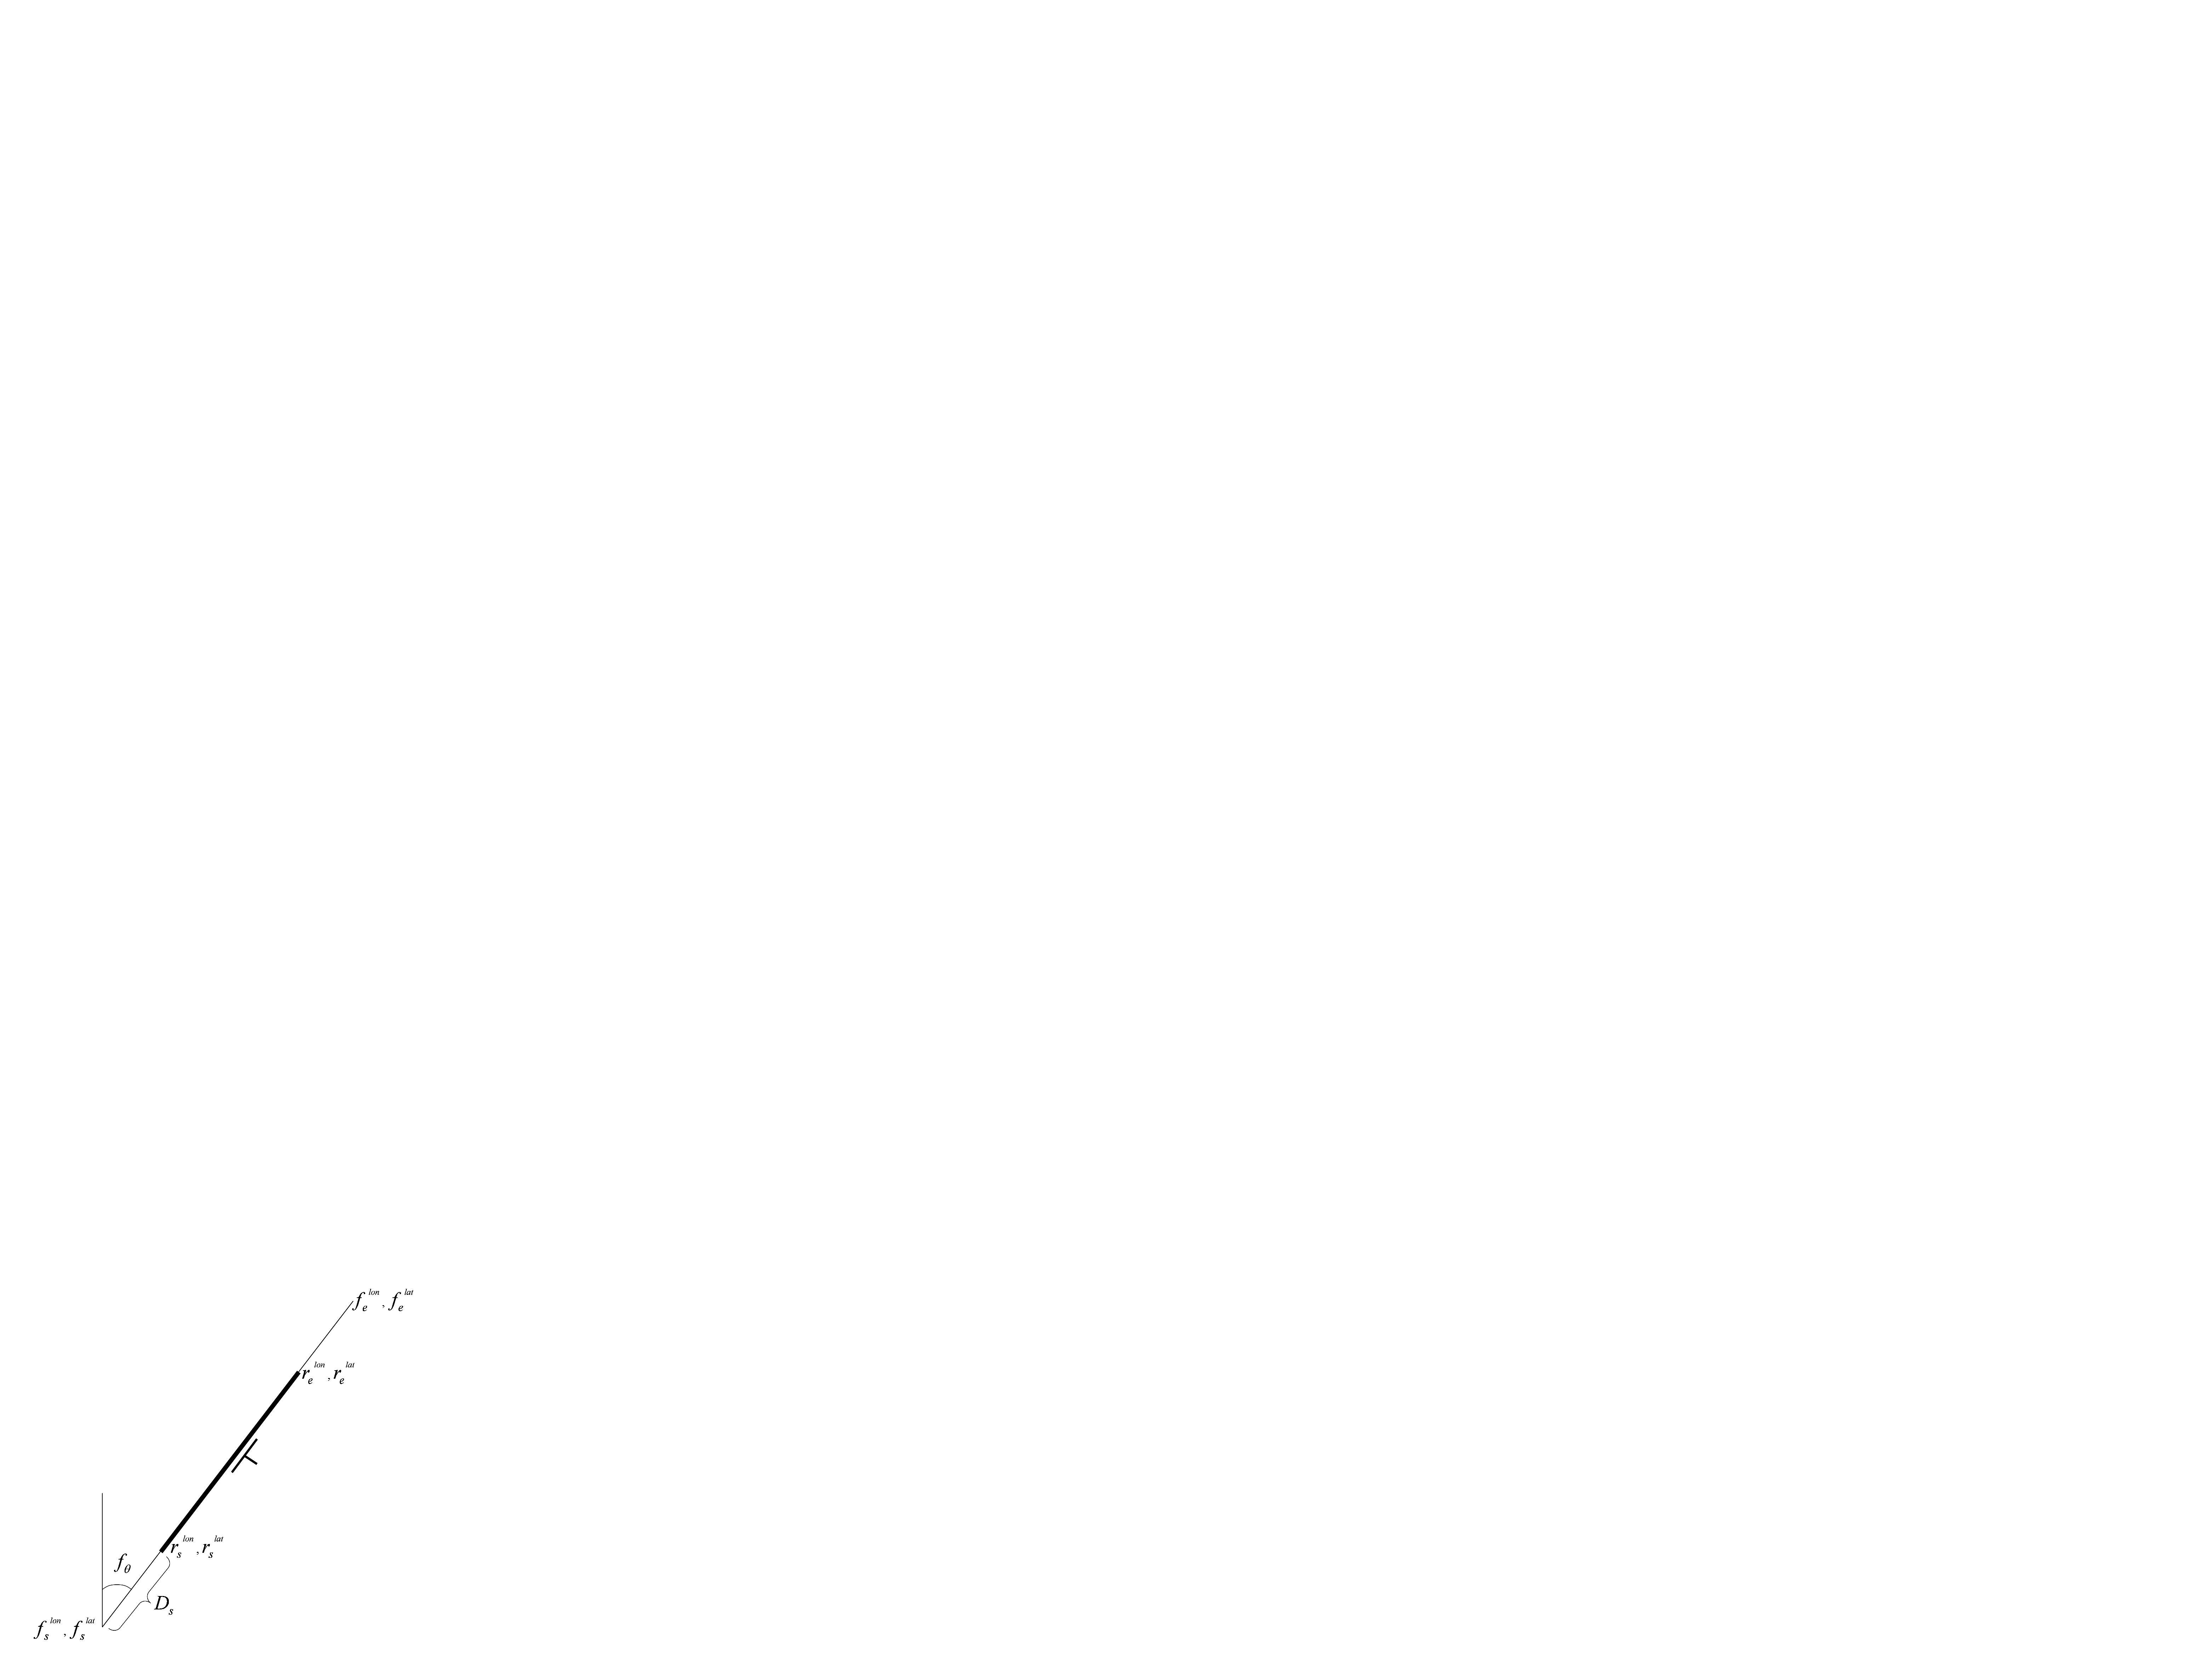
\includegraphics[width=12cm]
{fig-hsource-faulttrace}}
\caption{A plan view of the fault trace and rupture trace defined by its start and end coordinates.}
\label{fig:traces}
\end{figure}

A similar process to equation \ref{eq:ds} is followed to determine the depth of the rupture centroid (figure \ref{fig:rzrange}). 

\begin{figure}[htp]
\centerline{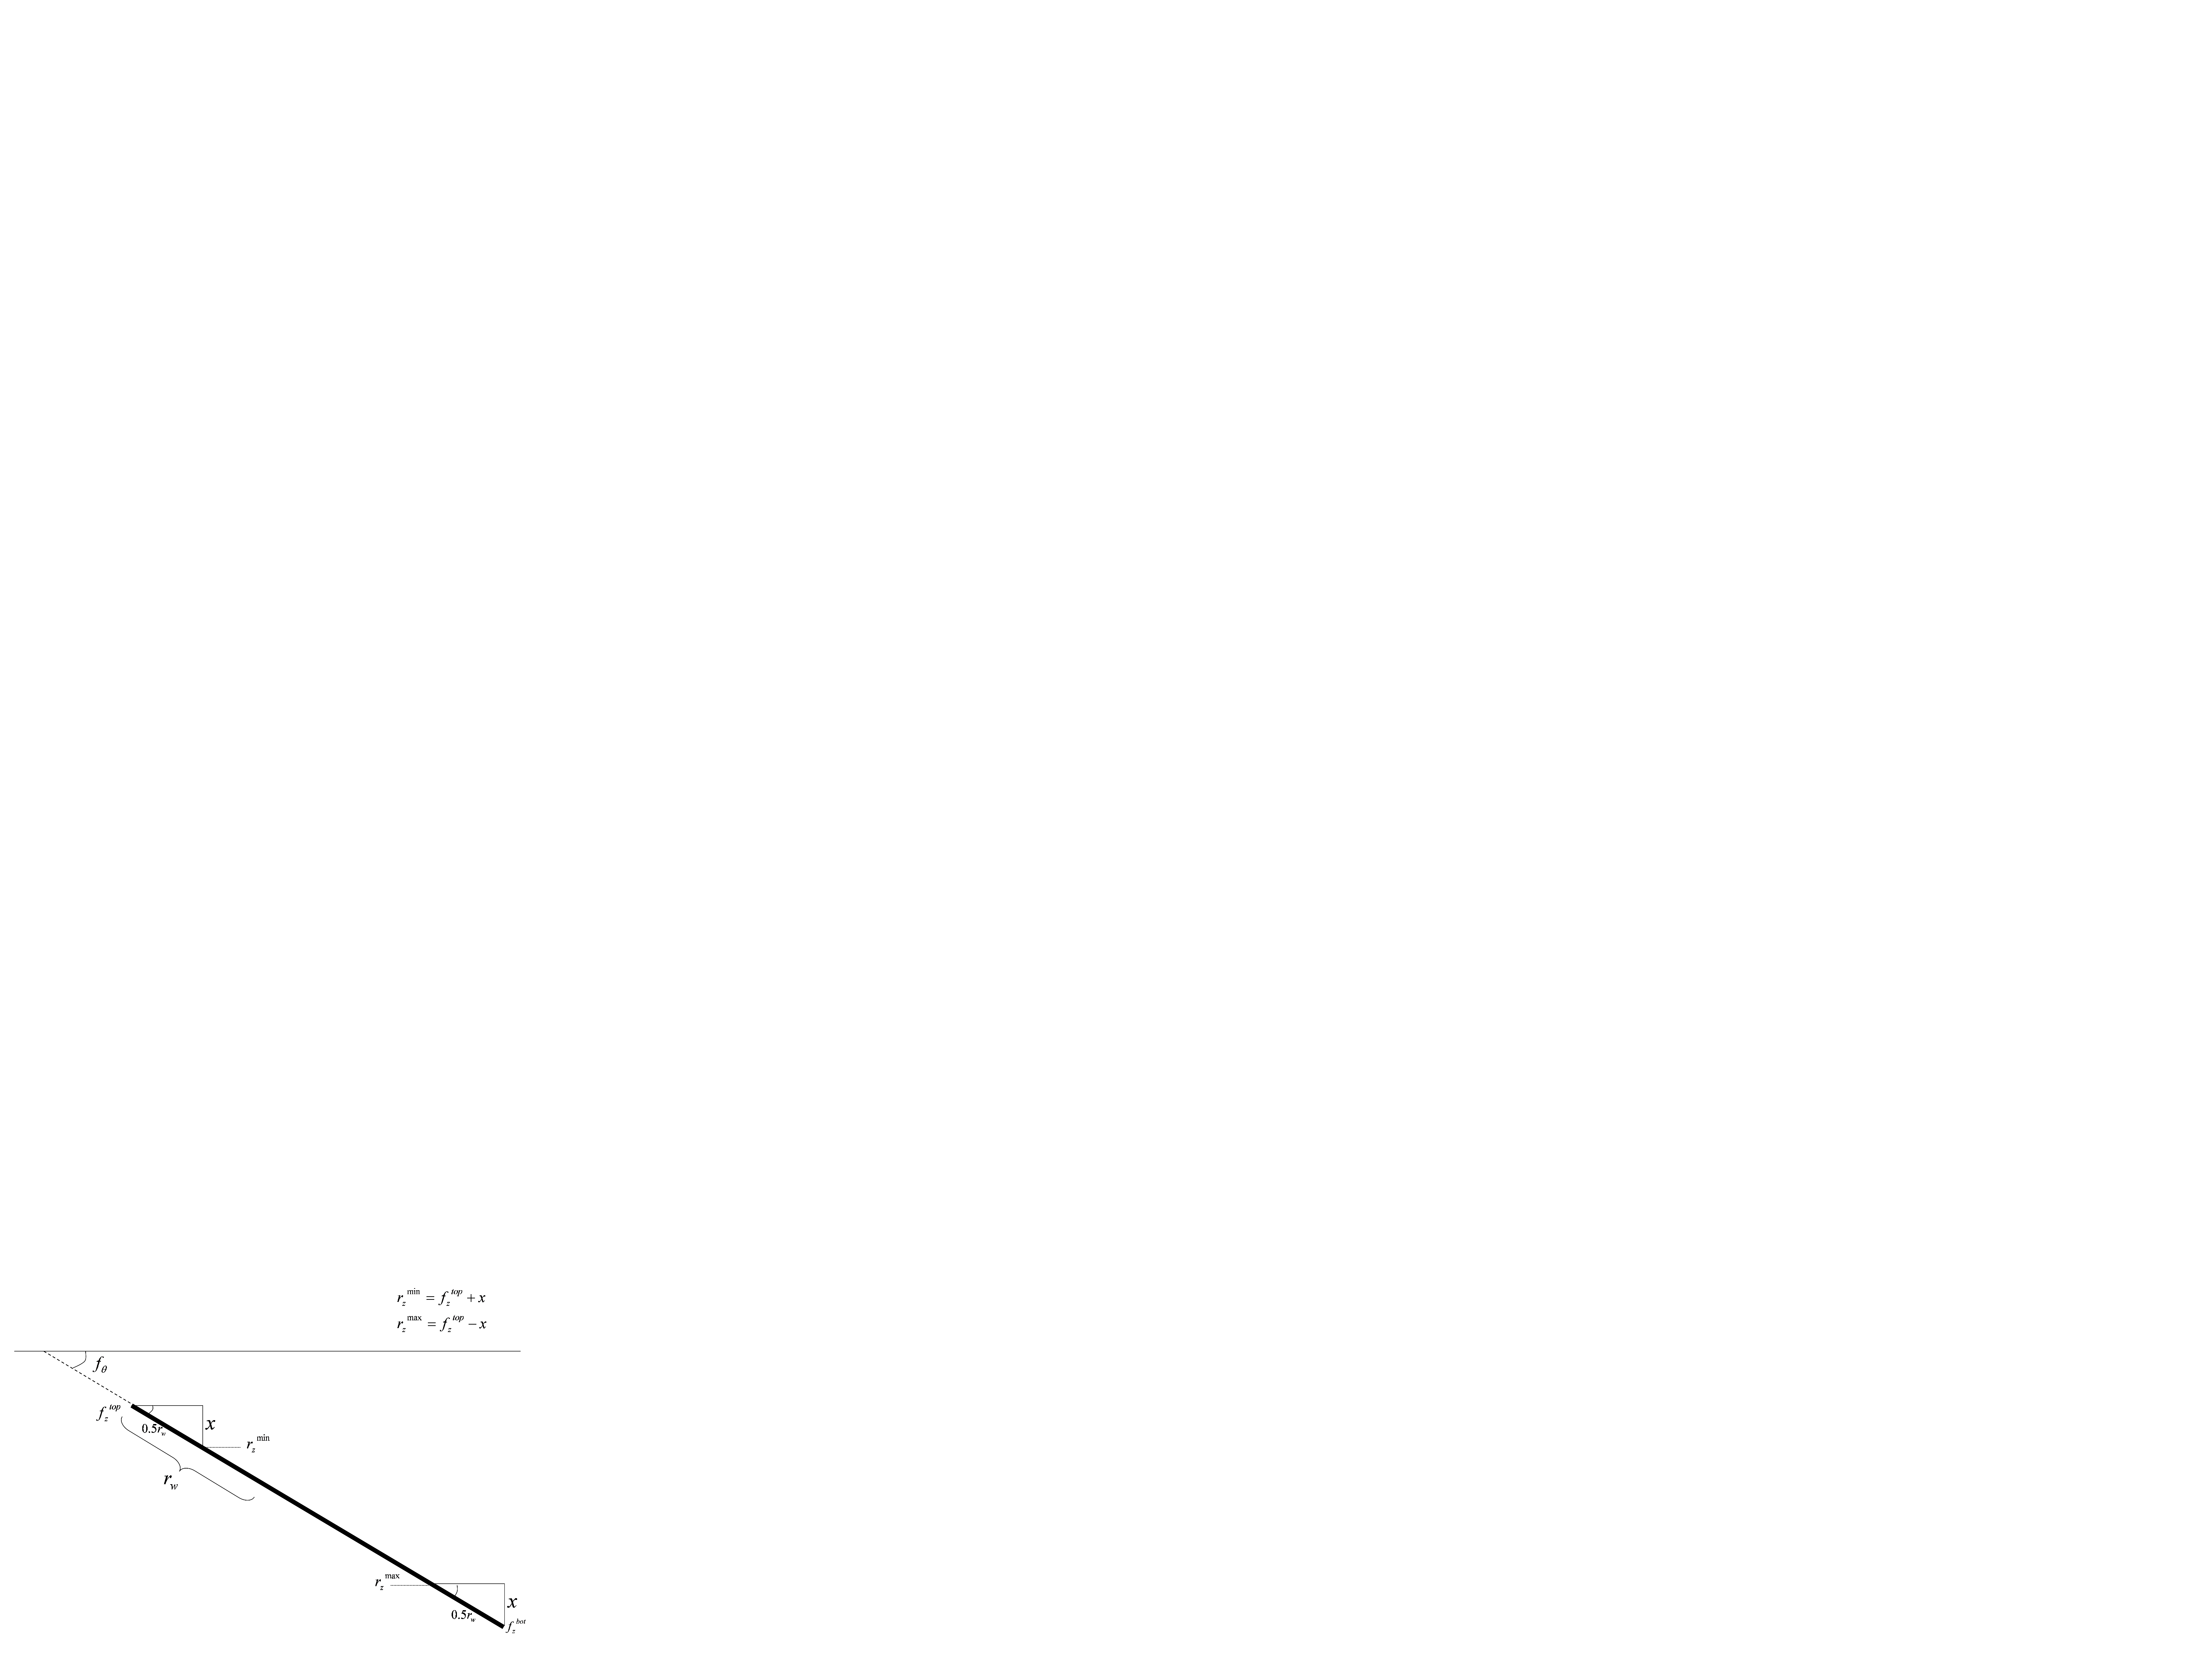
\includegraphics[width=12cm]
{fig-hsource-faultdepth}}
\caption{A schematic diagram of the depth range of the rupture centroid is calculated.}
\label{fig:rzrange}
\end{figure}

The depth range which the rupture centroid can lie within [$r_z^{min}, r_z^{max}$] such that 
the rupture plane does not extend above or below the bounds of the seismogenic zone [$f_z^{top}, f_z^{bot}$] is found from:

\begin{subequations} \label{drange}
\begin{align}
r_z^{min} & = r_z^{top} + 0.5r_w  \times sin(r_\theta)    \\
r_z^{max} & = r_z^{bot} - 0.5r_w  \times sin(r_\theta)  
\end{align}
\end{subequations}

where $f_\theta = r_\theta$. Note that for intraslab ruptures, which will be discussed later $f_\theta \ne r_\theta$. 
Now the rupture centroid depth is defined using a random uniform distribution between $r_z^{min}$ and $r_z^{max}$:

\begin{equation} \label{eq:rand}
	r_z = ( r_z^{max}-r_z^{min} ) \times  \mathtt{X} +   r_z^{min}
\end{equation}

where $\mathtt{X}$ is a random variable from 0$\rightarrow$1. The local x and y coordinates ($r_x$ and $r_y$) of the rupture 
centroid can be calculated by the employing the same equations as for the source zones:

\begin{equation}
r_y = r_z  \frac{cos(f_\theta)}{sin(f_\theta)}
\end{equation}

\begin{equation}
r_x = \frac{r_l}{2}
\end{equation}

Where the rupture centroid location in local coordinates ($r_x$, $r_y$) can be converted to longitude and latitude ($r_c^{lon}$, $r_c^{lat}$).

\subsection{Intraslab Faults}

The concept of creating realistic ruptures that represent events in a subducting slab is achieved by considering these events as 
out of plane ruptures. The subducting slab is defined as a 3D plane (centre of dipping slab) from which rupture planes extend out, at angles defined by
the user (figure \ref{fig:intraslabGeom}). This approach is restricted to using planar geometries, which is often not realistic on large scales. In which case 
a series of variably dipping or striking planes can be used to represent the curved dip of the intraslab. \\

For intraslab sources an out of dip value must be defined by the user($\delta_\theta$). 
This parameter defines the angle between the dipping plane and the rupture plane (figure \ref{fig:intraslabGeom}). If the rupture 
is parallel to the dipping plane $\delta_\theta$ will be zero. If the rupture plane is it an angle to the dipping plane then it 
will be non-zero. Another parameter, $\Delta_\theta$, defines the range of dips we will sample across to obtain the rupture 
dip ($r_\theta$, figure \ref{fig:intraslabGeom}).
A uniform sample is taken from the range [$\delta_\theta - \Delta_\theta, \delta_\theta + \Delta_\theta$] to determine 
the out of plane angle ($\omega$) and the dip of the rupture plane ($r_\theta$) :


\begin{equation}
\omega = 2\Delta_\theta  \times \mathtt{X} + \delta_\theta - \Delta_\theta
\end{equation}

where $\mathtt{X}$ is a random variable from 0$\rightarrow$1 and;

\begin{equation}
r_\theta = \omega + f_\theta
\end{equation}

When dealing with out of plane ruptures we need to consider three cases:
\begin{itemize} 
\item $0 \leq r_\theta \leq 90:$ \\ In this instance the rupture plane will dip in the same direction as the fault plane and we need to project the new rupture plane to 
the surface to define the surface trace of the rupture.
\item $90 <  r_\theta \leq 175:$ \\ In this case the rupture plane dips in the opposite direction to the fault plane and the local coordinate system must be transformed 
because the plane is no longer dipping to the right handside of the trace when looking from the start to the end of the trace. We must project the new rupture plane to 
the surface and then redefine the start and end locations of the rupture trace. This is because we always work in a right-handed local coordinate system with the rupture 
plane dipping to the right of the trace when looking along the trace from the start location to the end location (figure \ref{fig:intraslabGeom}).  
\item $185 < r_\theta \leq f_\theta + \omega :$ \\ In this case the rupture plane dips in the same direction of the fault plane, but the rupture trace is projected in 
the negative y direction of the local coordinate system. 
\end{itemize}

Note that since the EQRM uses the fault trace as a spatial reference, we force the rupture dip ($r_\theta$) to be 5$^\circ$ from horizontal (i.e. $r_\theta$ cannot lie 
between 175$^\circ$ and 185$^\circ$) so that the trace does not extend to infinity.

\begin{figure}[htp]
\centerline{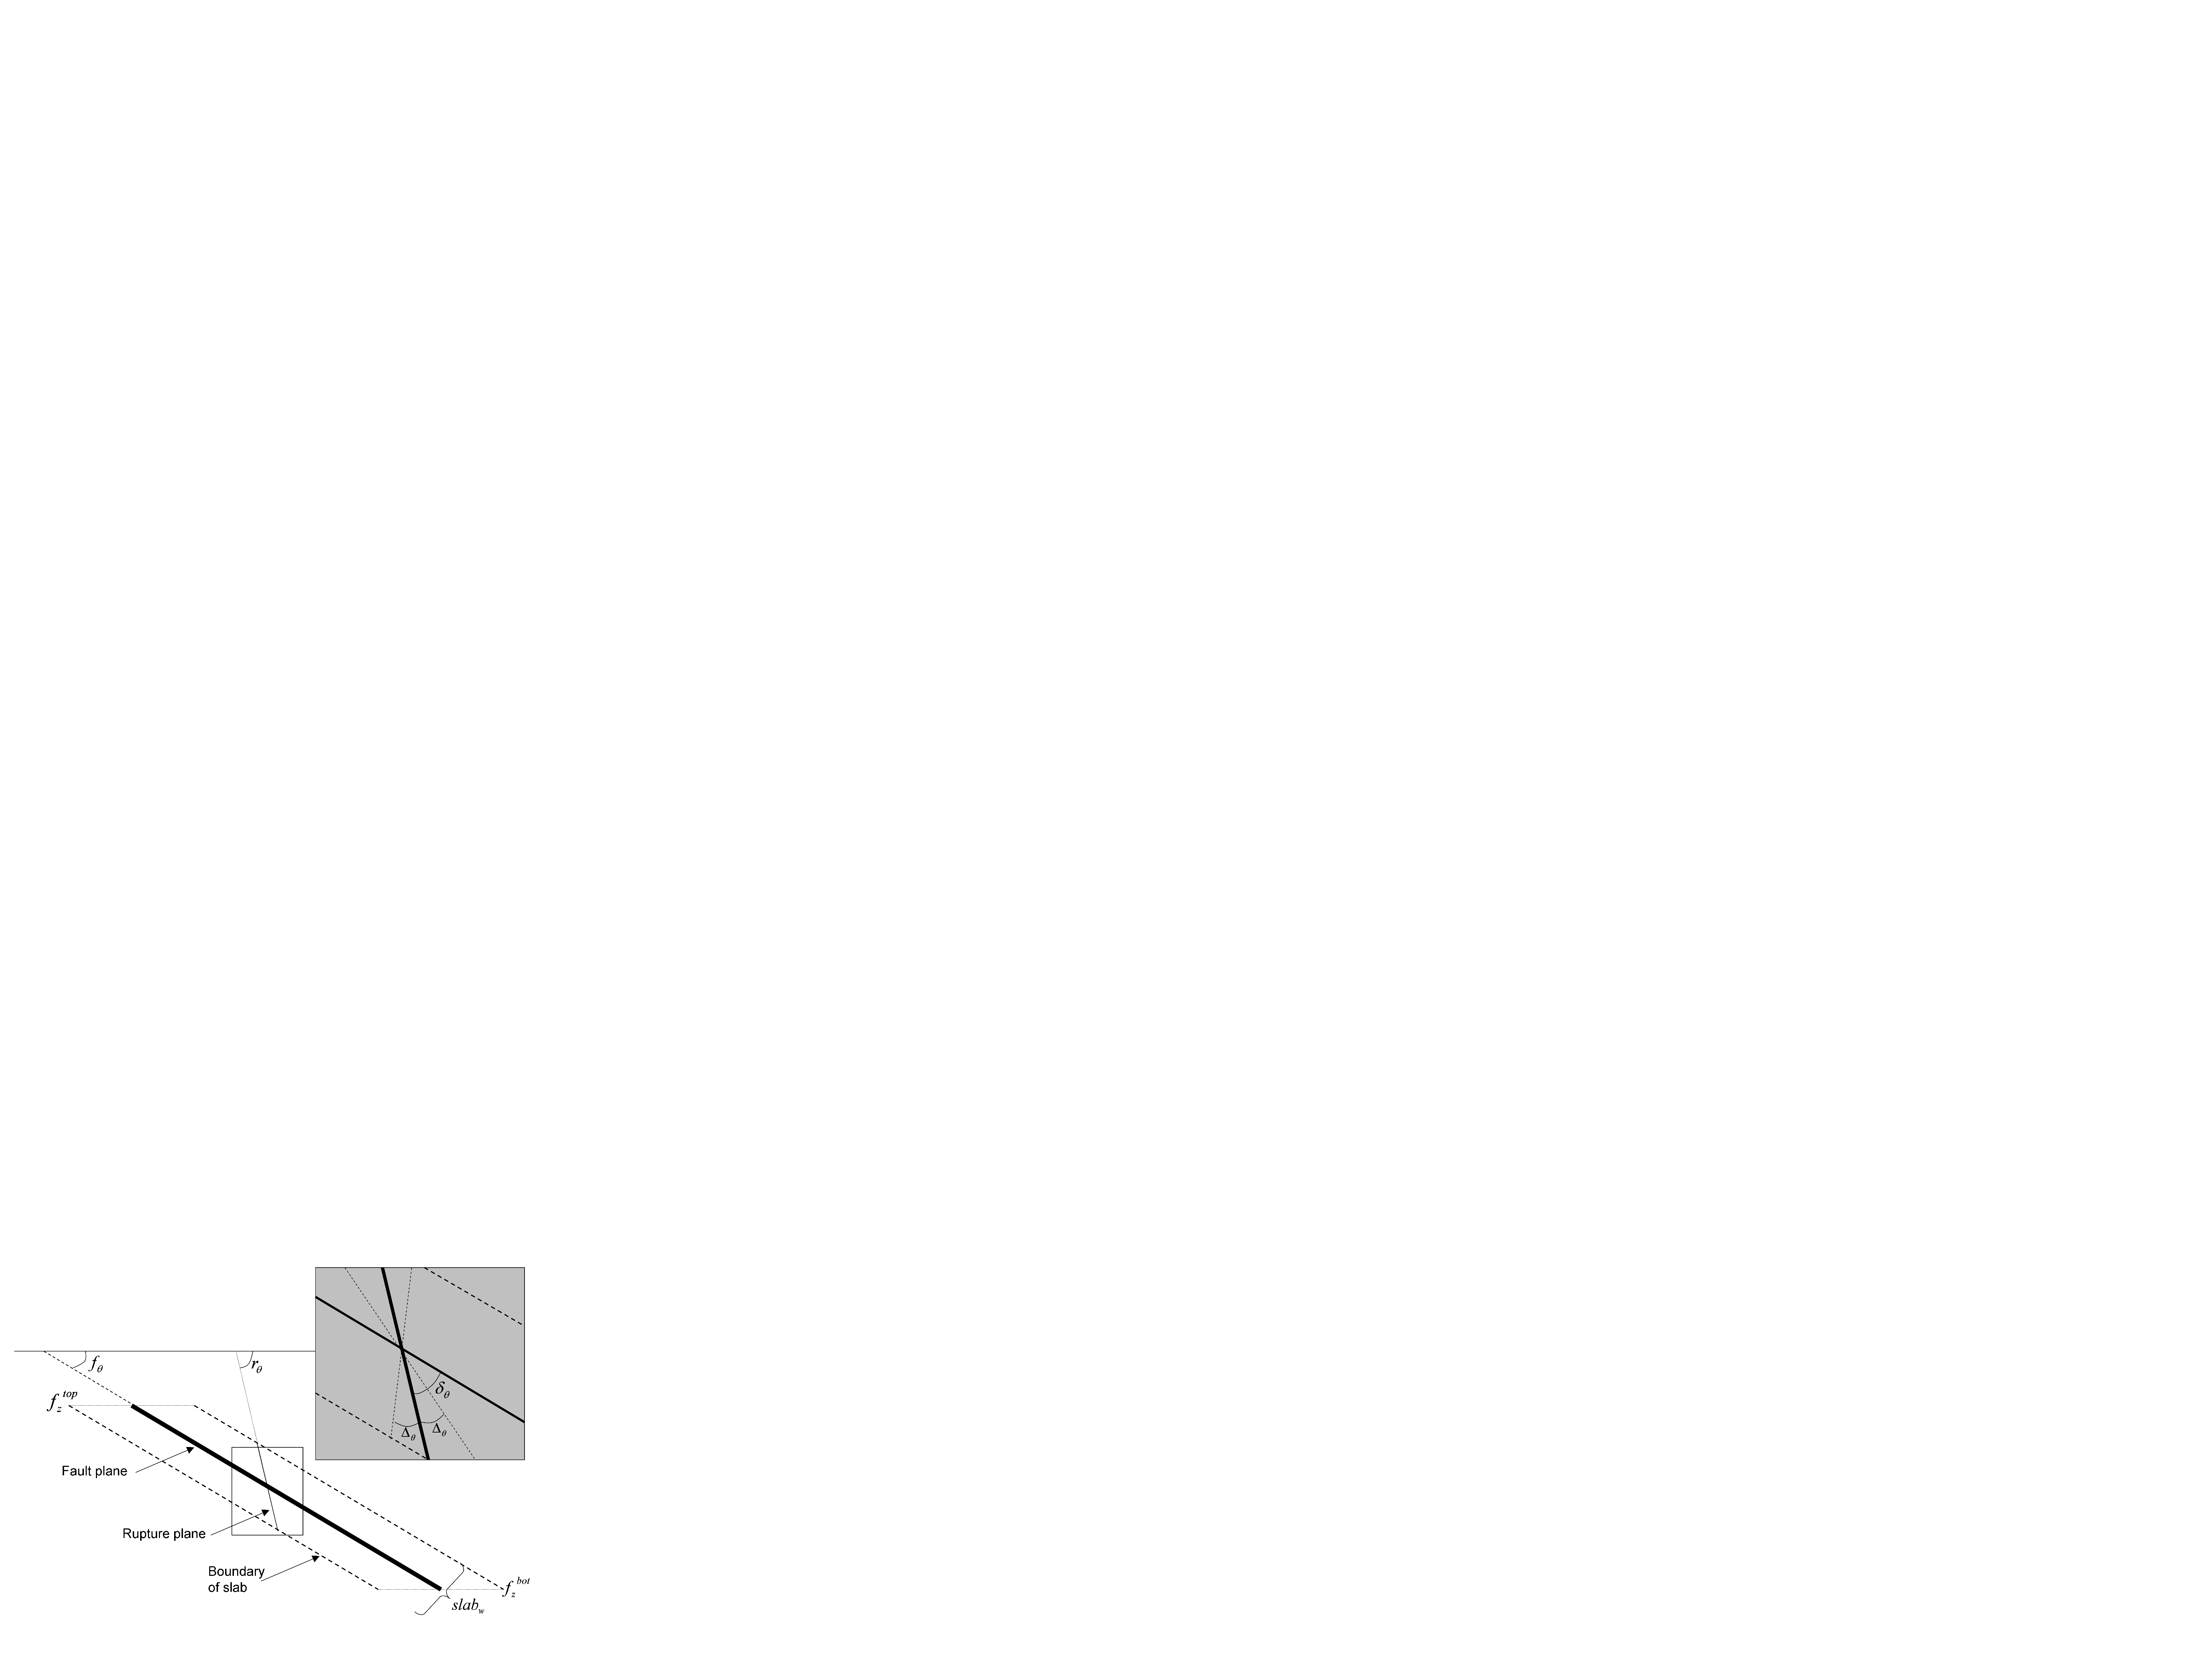
\includegraphics[width=16cm]
{fig-hsource-faultangles}}
\caption{A schematic diagram of the geometry of out of plane ruptures. This shows the rupture plane dipping out of the plane that defines the dipping slab. 
The inset is a zoom in of the angles that define the rupture plane geometry. The user defines the fault dip ($f_\theta$), which in this case represents the direction 
of the downgoing slab, and the out of plane dip ($\delta_\theta$) and a sampling range ($\Delta_\theta$) over which the EQRM will uniformly distribute the rupture plane. }
\label{fig:intraslabGeom}
\end{figure}

%%%%%
\subsubsection{Case if  $0 \leq r_\theta \leq 90$} \label{sec:0to90}
%%%%%

A similar approach to that in section \ref{sec:dim-rupture} is followed, where firstly the rupture plane dimensions (area $r_A$, width $r_w$ and length $r_l$) are defined. The rupture dimensions are forced to fall 
within the length of the fault, but this time it must not be allowed to extend outside of the width of the dipping slab ($S_w$) defined by the user. As shown in figure \ref{fig:deltaeq} the 
maximum width of the rupture plane ($r_w^{max}$) is found from:

\begin{equation}\label{rwmax}
r_w^{max} = 
\begin{cases}
 \frac{ S_w }{sin (\omega)}		& \quad \mbox{if $\omega$ $<$ 90} \\
S_w							& \quad \mbox{if $\omega$ $=$ 90} \\
 \frac{ S_w }{sin (180 - \omega ) }	& \quad \mbox{if $\omega$ $>$ 90} \\
\end{cases}
\end{equation}


\begin{figure}[htp]
\centerline{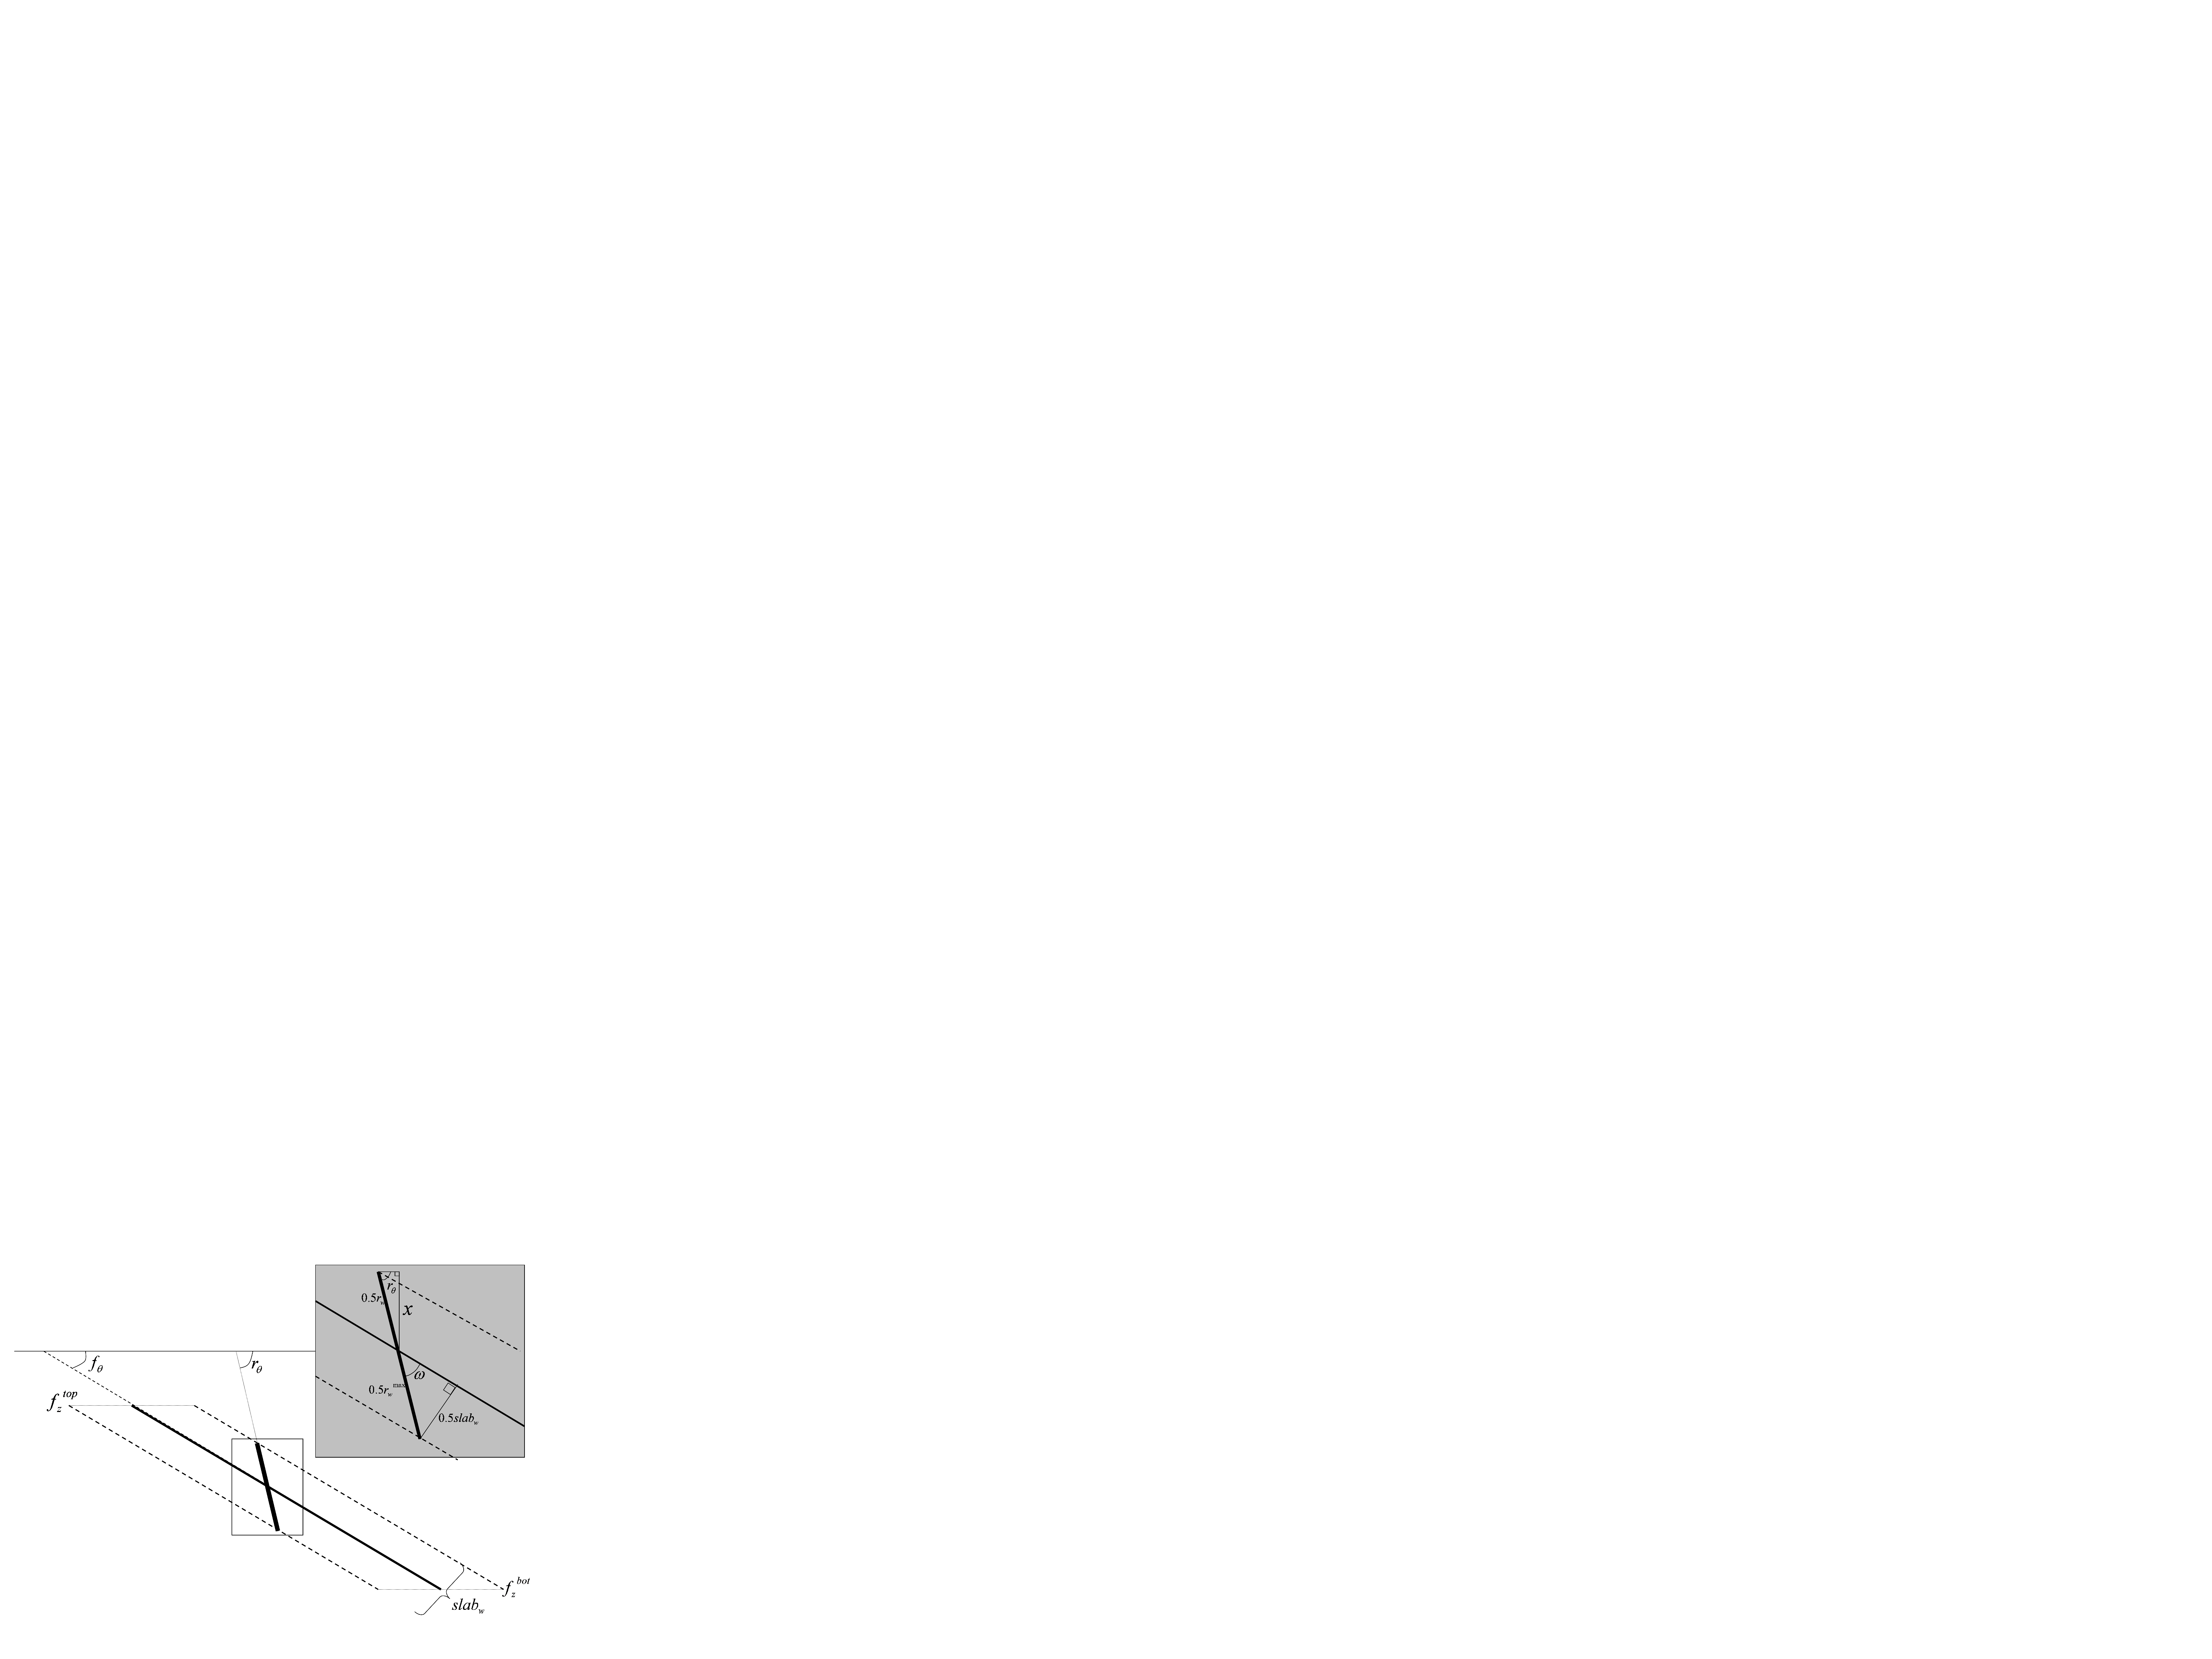
\includegraphics[width=12cm]
{fig-hsource-faultangles2}}
\caption{The geometry of determining the maximum rupture width ($r_w^{max}$) shown in the lower trigonometric geometry and the $r_z^{min}$ and $r_z^{max}$ shown in the upper part and equation \ref{drange2}.}
\label{fig:deltaeq}
\end{figure}

Equations \ref{ra} and \ref{eq:rw} are used to calculate the rupture area ($r_A$) and rupture width ($r_w^{WC}$) from the \citep{eqrm_Wells94} 
scaling laws. But for out of plane ruptures the rupture width ($r_w$) must be limited, not to the fault width as is the case 
of on plane ruptures, but to not extend beyond the slab boundary. Therefore a slightly modified version of 
equation \ref{eq:rw} is used to solve for the rupture width:

\begin{equation} \label{rw090}
r_w = \mathbf{min}\{ r_w^{WC}, r_w^{max}\}
\end{equation}

Now the rupture length ($r_l$) can be found, making sure it does not extend beyond the fault length ($f_l$) from:

\begin{equation}
r_l = \mathbf{min}\left\{\frac{r_A}{r_w}, f_l\right\}
\end{equation}

Equation \ref{eq:ds} is used to calculate $D_s$, the distance (km) along the fault trace for the start of rupture trace. Then the the position 
of the start and end of the rupture trace can be found. Note that we use new notation to describe the location of the start and end of the rupture trace along the 
fault trace ($\hat{r}_s^{lon}$, $\hat{r}_s^{lat}$, $\hat{r}_e^{lon}$, $\hat{r}_e^{lat}$). This is because the new location of the rupture 
trace ($r_s^{lon}$, $r_s^{lat}$ and $r_e^{lon}$, $r_e^{lat}$) will not be located along the original fault trace. 


Next the rupture centroid ($r_z$) depth range ($r_z^{min}$ to $r_z^{max}$) is defined, using a similar approach to that of equation \ref{drange}. This ensures 
the rupture trace does not go above or below the seismogenic zone of the fault. This is slightly different to equation \ref{drange} because the rupture 
plane is now dipping out of the fault plane (figure \ref{fig:deltaeq}).

\begin{subequations} \label{drange2}
\begin{align}
r_z^{min} & = f_z^{top} + 0.5r_w  \times sin(r_\theta)    \\
r_z^{max} & = f_z^{bot} - 0.5r_w  \times sin(r_\theta)  
\end{align}
\end{subequations}

Using equation \ref{eq:rand} we can now randomly assign the rupture centroid depth using a uniform distribution 
between $r_z^{min}$ and $r_z^{max}$:

\begin{equation}
r_z = ( r_z^{max}-r_z^{min} ) \times  \mathtt{X} +   r_z^{min}
\end{equation}

where $\mathtt{X}$ is a random variable from 0$\rightarrow$1. The rupture trace is projected to the surface to obtain the 
surface trace, and then to solve for the the rupture centroid. 
We begin by finding the location of the rupture centroid referenced to the start position of the original fault plane:

\begin{equation}\label{eq:ry}
\hat{r}_y = r_z  \frac{cos(f_\theta)}{sin(f_\theta)}
\end{equation}

and then:
\begin{equation}
\hat{r}_x = \frac{r_l}{2}
\end{equation}

Now the start ($\hat{r}_s^{x}$, $\hat{r}_s^{y}$) and end ($\hat{r}_e^{x}$, $\hat{r}_e^{y}$) position of the surface trace of the rupture plane can be calculated. This is done by first 
finding the location of the start location of the rupture ($r_s^{lon}$, $r_s^{lat}$) located along the fault 
plane in local coordinates. 

\begin{equation}\label{eq:rsx}
\hat{r}_s^{x} = 0
\end{equation}

then the dip of the rupture plane ($r_\theta$) is substituted into equation \ref{eq:ry}

\begin{equation}
\hat{r}_s^{y} = \hat{r}_y - r_z  \frac{cos(r_\theta)}{sin(r_\theta)}
\end{equation}

\begin{equation}\label{eq:rex}
\hat{r}_e^{x} = r_l
\end{equation}

\begin{equation}\label{eq:rey}
\hat{r}_e^{y} = \hat{r}_s^{y}
\end{equation}

The longitude and latitude for the start and end of the rupture trace can now be easily calculated.


All that remains is to redefine the location of the rupture centroid in local coordinates relative to the origin 
($r_s^{lon}$,$ r_s^{lat}$) of the new local coordinate system:
\begin{equation}\label{eq:rx}
r_x = 0.5 r_l
\end{equation}

\begin{equation} \label{eq:ry2}
r_y = r_z  \frac{cos(r_\theta)}{sin(r_\theta)}
\end{equation}

and then transform this into longitude and latitude. Note that $r_z = \hat{r}_z$.

%%%%%
\subsubsection{Case if $90 <  r_\theta \leq 175$} \label{sec:90t180}
%%%%%

In this instance the rupture plane is dipping in the opposite direction to the fault plane. Recall that if we look along 
the rupture trace the plane always dips to the right hand side, therefore in the case here of rupture plane the dips 
opposite to the project of the surface trace we need to re-project the rupture plane to the surface then swap the 
start and end coordinates. 


% $90 <  r_\theta \leq 180$

After calculating $r_w^{max}$ from equation \ref{rwmax} the $r_\theta$ must lie between 5 and 90. This limits flat ruptures which will have a rupture trace at infinity. The limit
of 5$^\circ$ was selected so coordinate transformation errors are not introduced when coverting between geographic and local systems due to the rupture trace being located at some
distance. 

\begin{equation}
r_\theta = \mathbf{max} \{ 180 - f_\theta + \omega, 5 \} .
\end{equation}


%\begin{equation}
%r_w^{max} = \frac{ slab_w }{sin ((180 - (r_\theta - f_\theta)) \times rad)}
%\end{equation}

\begin{figure}[htp]
\centerline{
\includegraphics[width=14cm]
{fig-hsource-faultflip}}
\caption{Fault and rupture plane geometry. Lower panel shows cross section view and upper panel shows a plan view of the surface 
projection. Note that in this case we need to re-project the rupture plane to the surface and redefine the start and end of the 
rupture trace such that the plane dips to the right hand side of the fault trace when looking from the start to end of the trace.}
\label{fig:gt90}
\end{figure}


The same approach is followed as section \ref{sec:0to90} from equations \ref{rw090} to \ref{eq:rsx}. However the next steps are slightly 
modified to add instead of subtract $r_y$ to the right handside of the equation: 

\begin{equation}
\hat{r}_s^{y} = \hat{r}_y + r_z  \frac{cos(r_\theta)}{sin(r_\theta)}
\end{equation}

And now the method in section \ref{sec:0to90} can again be followed from equations \ref{eq:rex} to \ref{eq:rey}. 
Again, the coordinate system must be transfored so the rupture start and end locations are swapped (Figure \ref{fig:gt180}).

Now the location of the rupture centroid is redefined in local x and y coordinates relative to the new 
origin ($r_s^{lon}$,$ r_s^{lat}$) of the new local coordinate system. The longitude and 
latitude of this point is then found using equations \ref{eq:rx} to \ref{eq:ry2}.

%%%%%
\subsubsection{Case if  $185 <  r_\theta \leq f_\theta + \omega$} \label{sec:180to270}
%%%%%

If the initial $r_\theta$ value is greater than 185 but less than $f_\theta + \omega$ then the rupture 
plane dips in the same direction of the fault plane but the rupture trace lies behind the fault trace (figure \ref{fig:gt180}). This is a case that requires different
treatment from above.

Again the dip of the rupture plane is forced to be greater than 5$^\circ$ so 
that the rupture trace projects to the surface:

\begin{equation}
r_\theta = \mathbf{max} \{ 180 - f_\theta + \omega, 5 \} .
\end{equation}

\begin{figure}[htp]
\centerline{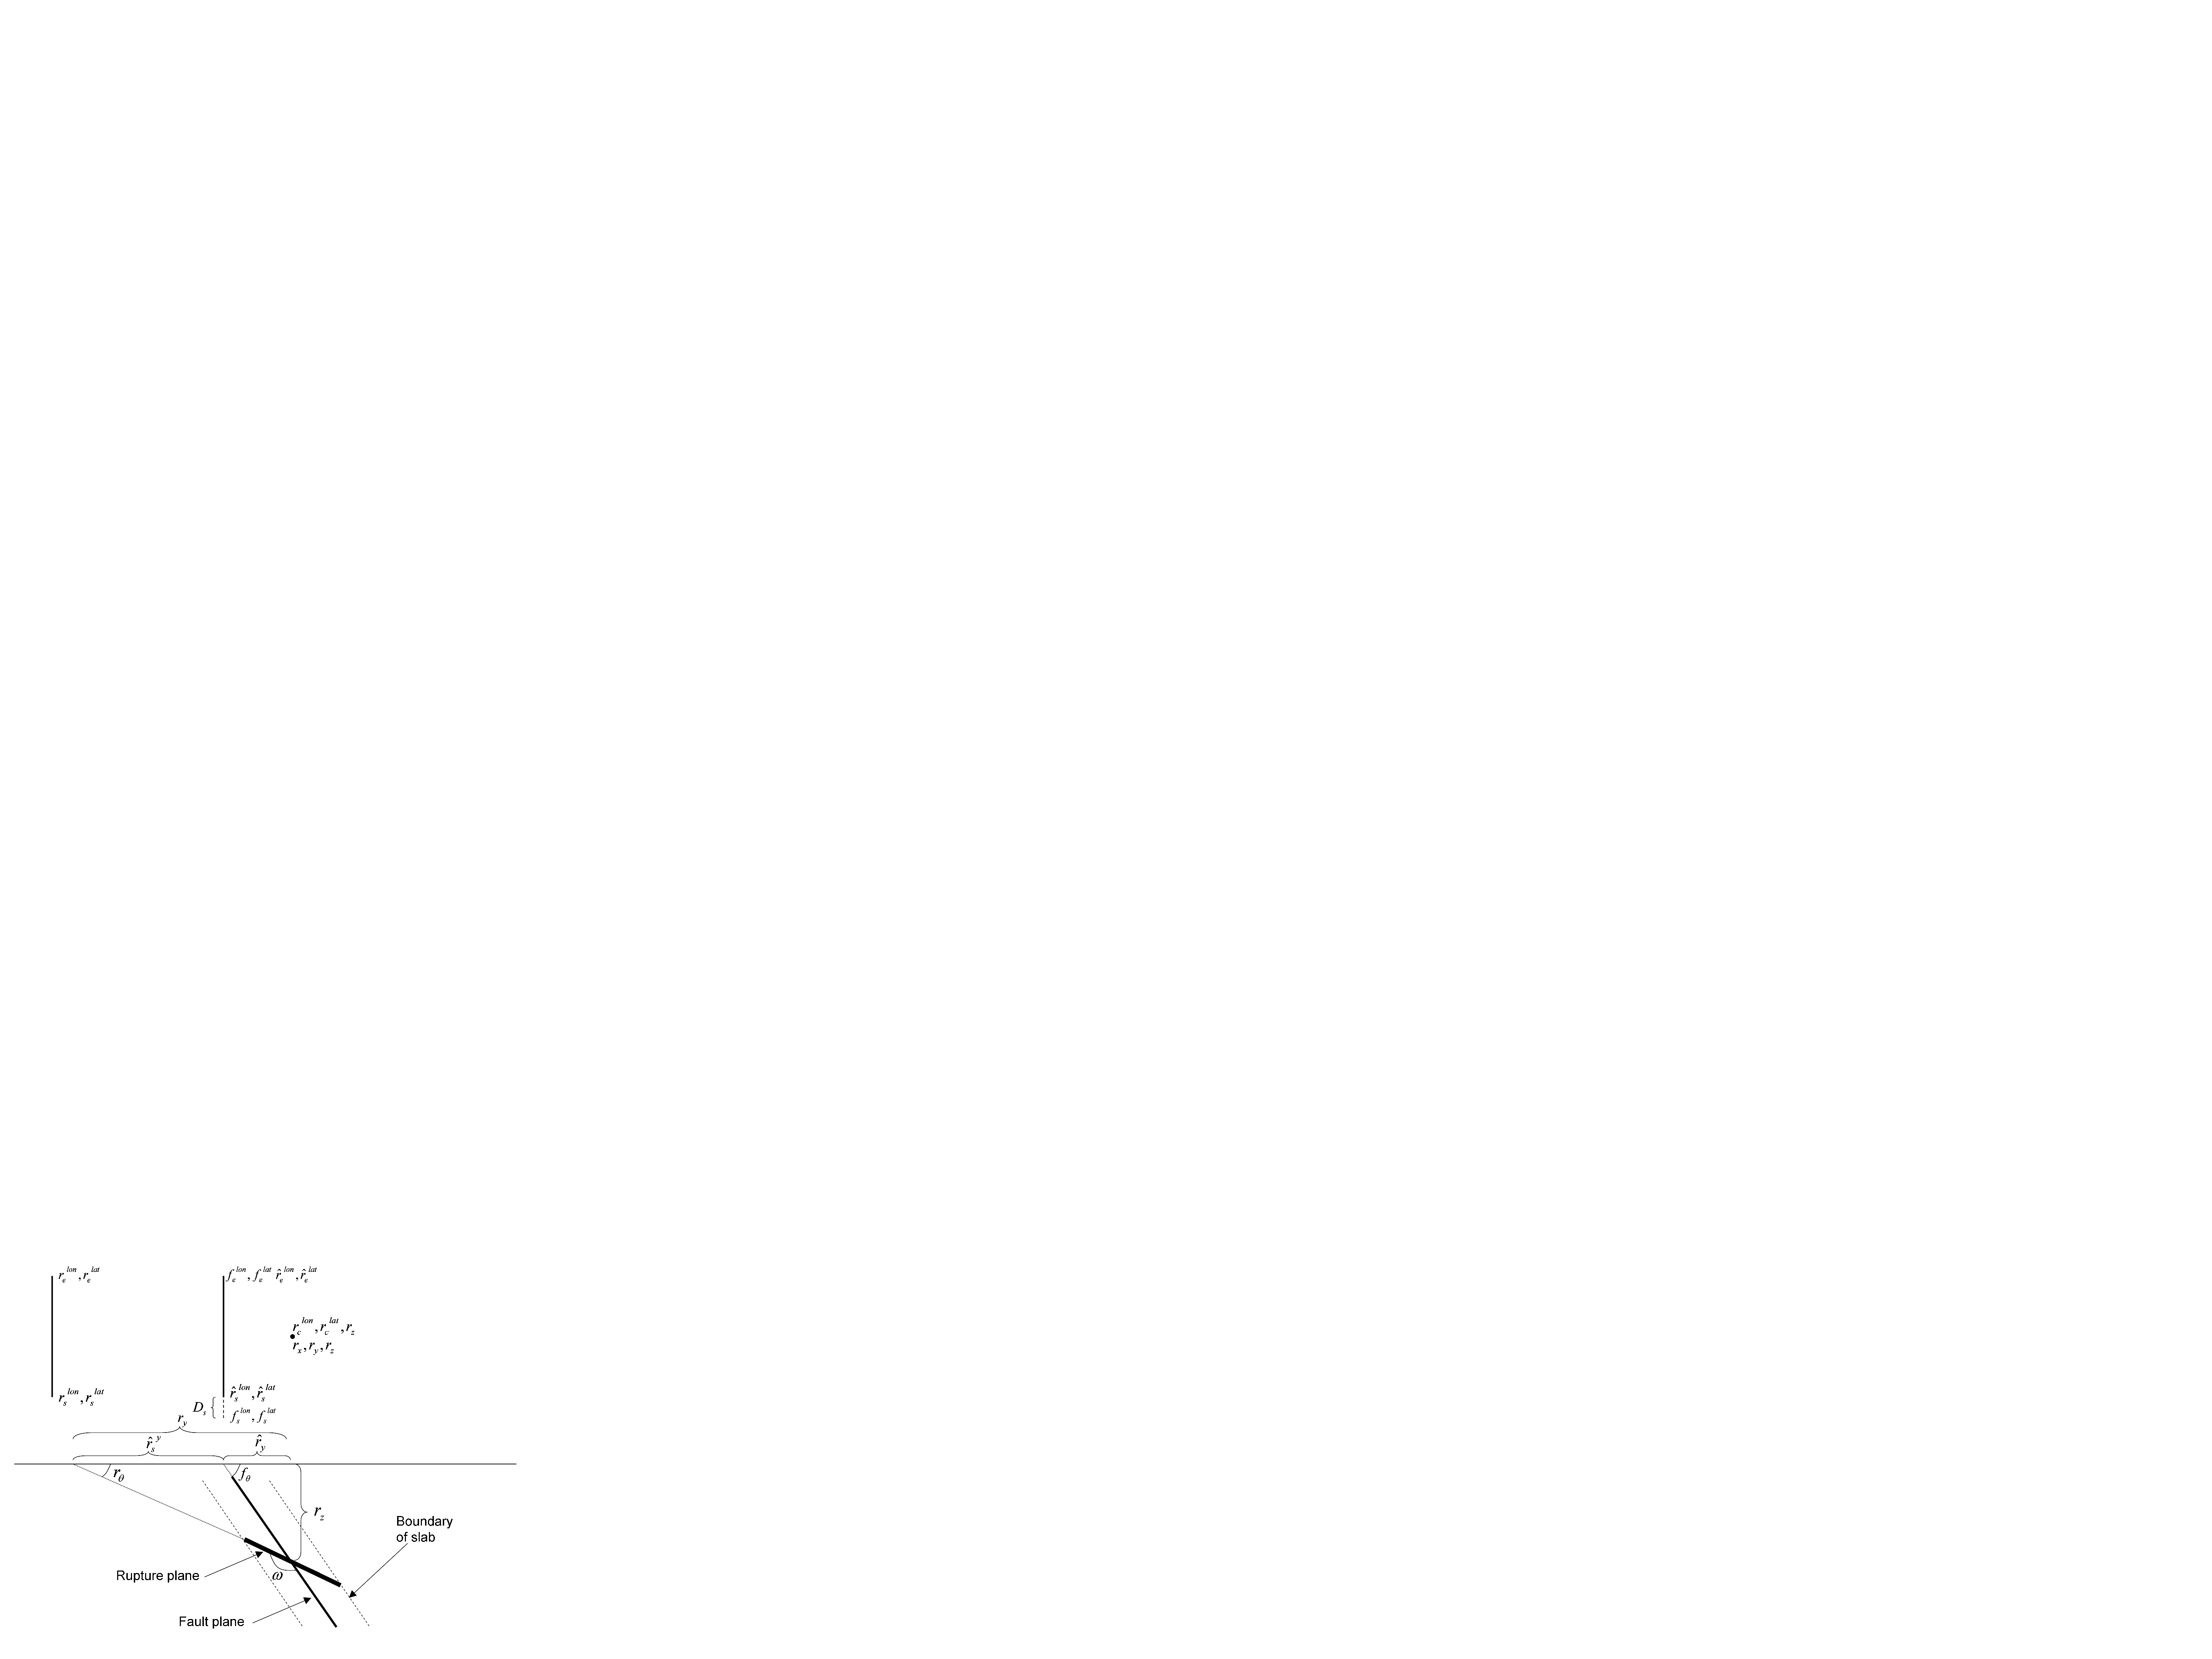
\includegraphics[width=14cm]
{fig-hsource-faultflipbehind}}
\caption{Fault and rupture plane geometry for. Lower panel shows cross section view and upper panel shows 
a plan view of the surface projection. Note that in this case we need to re-project the rupture plane to 
the surface and redefine the start and end of the rupture trace.}
\label{fig:gt180}
\end{figure}

The same methods as above, until equation \ref{eq:rsx} are used but now the following equation must be modified
to solve for ($\hat{r}_y$) which in this case will be negative:

\begin{equation}\label{eq:ry4}
\hat{r}_s^y = \hat{r}_y -  r_z  \frac{cos(r_\theta)}{sin(r_\theta)}.
\end{equation}

The end of the rupture trace in local coordinates ($\hat{r}_e^x$ and $\hat{r}_e^y$) referenced to the fault 
trace can be found from:
\begin{equation}
\hat{r}_e^x = r_l
\end{equation}

\begin{equation}
\hat{r}_e^y = \hat{r}_s^y
\end{equation}

These local coordinates can now be converted to latitude and longitude using the local reference system. 


\section{Spawning events}
\label{source:spawning}


There is an option within the EQRM application to spawn (or copy)
events. Such copies are required by some techniques for
incorporating aleatory uncertainty in later stages of the PSHA and
PSRA. For example, \sref{attn:uncert-randomchoice} describes an
incorporation of aleatory attenuation uncertainty that does not
require spawning of the catalogue whereas
\sref{attn:uncert-pdfchoice} describes a process that does require
spawning. 

When spawning the weight $w_e$ is derived by
truncating and re-normalising a standard normal distribution to
$\pm n_\sigma$. The process is summarised below.

We know that the standard normal distribution $ N \sim (0,1)$ has
a PDF given by
\begin{equation}
\begin{array}{lr}
f_X(x)=\frac{1}{\sqrt{2\pi}}e^{\frac{-x^2}{2}} & - \infty <x<
\infty.
\\
\end{array}
\end{equation}

To truncate and re-normalise $N \sim (0,1)$ to $\pm n_\sigma$ we
must evaluate $P(-n_\sigma \sigma \leq X \leq n_\sigma \sigma)$.
The error function
\begin{equation}
erf(x) = \frac{2}{\sqrt{\pi}} \int_{0}^{x} e^{-t^2} \, dt.
\end{equation}
is related to the cumulative area under the standard normal
distribution via
\begin{equation}
erf(x) = 2P(X \leq x)-1.
\end{equation}
Then $P(-n_\sigma
\sigma \leq X \leq n_\sigma \sigma)$ is comptued using the error function as
follows
\begin{equation}
\begin{array}{rcl}
P(-n_\sigma \sigma \leq X \leq n_\sigma\ \sigma)  & = & P(X \leq
n_\sigma)-P(X \leq -n_\sigma) \\
   & = & 2P(X \leq n_\sigma)-1 \\
    & = & erf(n_\sigma) . \\
\end{array}
\end{equation}

Following this we compute the truncated and
re-normalised PDF by evaluating
\begin{equation}
\begin{array}{lr}
\tilde{f}_X(x)= \frac{1}{P(-n_\sigma \sigma \leq X \leq n_\sigma
\sigma)}
\frac{1}{\sqrt{2\pi}}e^{ \frac{-x^2}{2}} & -n_\sigma \sigma <x< n_\sigma \sigma. \\
\end{array}
\end{equation}

The observant reader will notice that because the EQRM application
works in the discrete world, simply evaluating $\tilde{f}_X(x)$
will not suffice. The approach used 
to discretise $\tilde{f}_X$ and compute the weights
$\{w_{e,i}\}_{i=1}^{n_{samples}}$ is identical to that used to
compute the event activity $r_\nu$ (see
\sref{sec:magnitude_selection}). That is
\begin{equation}
w_{e,i} = \frac{\tilde{f}_X(x_i)}{\sum\limits_{j=1}^{n_{samples}}
\tilde{f}_X(x_j)}.
\end{equation}
Once the weights $\{w_{e,i}\}_{i=1}^{n_{samples}}$ are computed
the event activity $r_\nu$ for each of the event copies is
re-defined as follows:
\begin{equation}
\label{source:spawning-activity}
\begin{array}{ll}
r_{\nu,i} = r_{\nu,original} \times w_{e,i} & \textrm{for } i=1
\textrm{ to } n_{samples},
\end{array}
\end{equation}
for each copy of the original event and its associated weighting.
A source epsilon term $r_\varepsilon$ is also defined for each
copy of the original event i.e.
$\{r_{\varepsilon,i}\}_{i=1}^{n_{samples}}$. Each of the
$r_{\varepsilon,i}$ are defined such that they correspond to the
$i^{th}$ bin centroid from the $n_{samples}$ bin spanning $\pm
n_\sigma$ (see \sref{attn:uncert-pdfchoice} for the mathematical
definition).


\section{Analysing a scenario event}
\label{sec:source-scenario} 
The EQRM application incorporates an option for considering
a particular (or scenario) event. The earthquake parameters needed take the same
form as that described in \tref{tab:parameters}. The scenario
event is constrained by user defined values for magnitude, rupture centroid,
depth and azimuth. The length and width are calculated using the \citet{eqrm_Wells94} scaling laws.




%%% Local Variables:
%%% mode: latex
%%% TeX-master: "eqrmtech"
%%% End:
